
%_____________________________________________________________________________
%=============================================================================
% main.tex v8 (31-05-2015) \ldots dibuat oleh Lionov - Informatika FTIS UNPAR
% 
% Ini adalah file utama (main.tex), berisi perintah-perintah yang khusus 
% dibuat untuk template ini
%
% 			JANGAN MENGUBAH APAPUN DI DALAM FILE INI,
%			KECUALI ANDA TAHU APA YANG ANDA LAKUKAN !!!
%
% Jika ada tambahan perintah, dapat anda tuliskan di tempat yang telah disediakan 
% di baris 310 pada file ini
% Jika daftar tabel tidak digunakan, anda harus menghapus (beri komentar) secara
% manual di baris 485
%
% Bug, kritik, saran: silahkan kirimkan via email ke lionov@unpar.ac.id
%
% Perubahan pada versi 8 (31-05-2015):
%	- penambahan default data untuk beberapa keterangan dan digunakan sebagai 
%	  template dengan tanda << & >> . Data yang diubah defaultnya adalah: nama skripsi
%	  nama prodi, beserta bahasa inggrisnya.
%   - Keywords dan kata kunci di abstrak ditambahkan noindent + perbaikan lainnya
%   - Perbaikan untuk halaman tidak kosong tanpa nomor halaman romawi
%

% Perubahan pada versi sebelumnya :
%	versi 7 (27-05-2014)
%	- penambahan perintah \raggedbottom untuk menghilangkan area kosong akibat 
%	  penempatan gambar yang tidak sempurna
%	versi 6 (10-11-2013)
%	- perbaikan pada abstract dengan paragraf lebih dari satu: perbaikan vertical spacing
%	- perbaikan pada tampilan bab dan lampiran: tidak perlu menuliskan apapun untuk 
%	  menampilkan semuanya (di data.tex) atau -1 jika tidak ada lampiran
%	- halaman bernomor genap untuk halaman romawi sudah dimunculkan
%	- Kurikulum 2013 : perubahan nama buku skripsi 
%	versi 5 (21-10-2012)
%	- halaman terakhir setiap bab tidak ada headernya jika kosong
%	versi 4 (06-08-2012)
% 	- penggabungan main.tex, depan.tex dan setup.tex menjadi main.tex
% 	- menambahkan keterangan di lampiran untuk kode program 
% 	- ukuran font dapat diubah langsung di tiap lampiran
% 	versi 3 (09-07-2012): 
%	- Tidak ada di file ini
% 	versi 2 :
% 	- "Daftar Referensi" tidak perlu diubah secara manual (tidak perlu mengubah file bahasai.ldf)
% 	- Bahasa Indonesia dari abstract adalah abstrak (secara otomatis), bukan ringkasan
% 	- Spasi pada buku dokumen final adalah onehalfspacing
%
% to do : - hilangkan secara otomatis daftar tabel/gambar jika tidak digunakan
%         - (IT) aturan penulisan algoritma untuk IT (pakai algo.sty ?)
%=============================================================================

%=============================================================================
% setup.tex v2 (08-07-2012)
% Perubahan pada versi 2:
% - Menambahkan perintah untuk judulINA dan judulENG
% - Menghapus \usepackage{microtype}, yang pada beberapa kasus menjadi masalah
%=============================================================================
% depan.tex v2 (09-07-2012)
% Perubahan pada versi 2:
% - Menambahkan halaman depan dalam bahasa inggris
%=============================================================================

%setup.tex
\documentclass[11pt,a4paper,twoside,openright,notitlepage]{report} 

\usepackage[bahasa]{babel} %bahasa indonesia
\usepackage[T1]{fontenc}  %encoding
% \usepackage{mathptmx}
% \usepackage{venturisold}
% \usepackage{helvet}
% \usepackage{fouriernc} 
\usepackage{abstract} %manipulasi abstract
\usepackage{chappg} % format daftar isi 
\usepackage{color} %warna
\usepackage{etoolbox} %untuk programming if-then
\usepackage{fancyhdr} %format header & footer
\usepackage{float} %penempatan gambar di tempat yg seharusnya
\usepackage[inner=2.5cm,outer=2cm,top=2.5cm,bottom=2.5cm]{geometry} %margin
\usepackage{graphicx} %gambar
\usepackage{listings} %source code
\usepackage{lscape} %landscape untuk source code
\usepackage{multicol} %multiple column
\usepackage{ifthen} % if then
\usepackage[pagewise]{lineno} %line numbering
\usepackage{lipsum} % untuk testing
\usepackage{titlesec} %judul header
\usepackage{tocbibind} %daftar isi, gambar, tabel dll
\usepackage{tocloft} % format daftar isi 
\usepackage{setspace} %line spacing
\usepackage{xstring} %manipulasi string
\usepackage[plainpages=false,pdfpagelabels,unicode]{hyperref} %\autoref, \phantomsection & link 
\usepackage{emptypage}

\let\abstractname\Abstrak

\titleformat{\chapter}[display] {\Large\bfseries\centering}{\MakeUppercase{\chaptertitlename} \thechapter}{15pt}{\Large\MakeUppercase}

\renewcommand{\cftchapfont}{\scshape \bfseries}

\renewcommand{\cfttoctitlefont}{\hfill\Large\bfseries\MakeUppercase}
\renewcommand{\cftaftertoctitle}{\hfill}
\renewcommand{\cftloftitlefont}{\hfill\Large\bfseries\MakeUppercase}
\renewcommand{\cftafterloftitle}{\hfill}
\renewcommand{\cftlottitlefont}{\hfill\Large\bfseries\MakeUppercase}
\renewcommand{\cftafterlottitle}{\hfill}

% Tidak perlu ada kata "Bab", "Gambar" atau "Tabel" di daftar 
% \renewcommand{\cftchappresnum}{{\bf \scshape Bab} } 
% \renewcommand{\cftchapnumwidth}{1.5cm}
% \renewcommand{\cftfigpresnum}{{Gambar\ }} 
% \renewcommand{\cftfignumwidth}{2.5cm}
% \renewcommand{\cfttabpresnum}{{Tabel\ }} 
% \renewcommand{\cfttabnumwidth}{2cm}

\newcommand{\apptoc}{
	% Hapus kata "Lampiran" dari daftar isi
	%\addtocontents{toc}{\protect\renewcommand{\protect\cftchappresnum}{\bf \scshape Lampiran\  }}%
	%\addtocontents{toc}{\protect\renewcommand{\protect\cftchapnumwidth}{2.75cm}}
	\addtocontents{toc}{\protect\renewcommand{\protect\cftchappresnum}{\bf \scshape}}%	

}

\newcommand{\vnama}{Jane Doe}
\newcommand{\vlnama}{John Doe}
\newcommand{\vnpm}{1992700001}
\newcommand{\vprodiINA}{SAINS}
\newcommand{\vprodiENG}{SCIENCE}
\newcommand{\vstaINA}{UJIAN}
\newcommand{\vstaENG}{EXAM}
%\newcommand{\vjudul}{Judul Skripsi/Tugas Akhir}
\newcommand{\vpembu}{Plato}
\newcommand{\vpembs}{Euclid}
\newcommand{\vpengi}{Plato}
\newcommand{\vpengii}{Euclid}
\newcommand{\vtanggal}{1}
\newcommand{\vbulan}{Januari}
\newcommand{\vtahun}{1970}
\newcommand{\vmode}{final}
\newcommand{\vspacing}{double}
\newcommand{\vlineno}{yes}
\newcommand{\vkunciina}{Skripsi, Tugas Akhir}
\newcommand{\vkuncieng}{Undergraduate Thesis, Final Project}
\newcommand{\vkajur}{Jack Doe}
\newcommand{\vkajurmat}{Jack Doe}
\newcommand{\vkajurfis}{Jack Doe}
\newcommand{\vkajurtif}{Jack Doe}

\newcommand{\namanpm}[2]{
	\renewcommand{\vstaINA}{<<SKRIPSI/TUGAS AKHIR>>}
	\renewcommand{\vprodiINA}{<<MATEMATIKA/FISIKA/TEKNIK INFORMATIKA>>}
	\renewcommand{\vstaENG}{<<FINAL PROJECT/UNDERGRADUATE THESIS>>}
	\renewcommand{\vprodiENG}{<<MATHEMATICS/PHYSICS/INFORMATICS>>}
	\renewcommand{\vnama}{\uppercase{#1}} \renewcommand{\vlnama}{#1} \hypersetup{pdfauthor={#2 - #1}}
	\renewcommand{\vnpm}{#2} \hypersetup{pdfcreator={#2}} \StrChar{\vnpm}{6}[\vprodiN]
	\ifdefstring{\vprodiN}{1}{
		\renewcommand{\vprodiINA}{MATEMATIKA} \renewcommand{\vprodiENG}{MATHEMATICS} 
		\renewcommand{\vstaINA}{SKRIPSI} \renewcommand{\vstaENG}{FINAL PROJECT} \renewcommand{\vkajur}{\vkajurmat}}{}
	\ifdefstring{\vprodiN}{2}{
		\renewcommand{\vprodiINA}{FISIKA} \renewcommand{\vprodiENG}{PHYSICS} 
		\renewcommand{\vstaINA}{TUGAS AKHIR} \renewcommand{\vstaENG}{FINAL PROJECT} \renewcommand{\vkajur}{\vkajurfis}}{}
	\ifdefstring{\vprodiN}{3}{
		\renewcommand{\vprodiINA}{TEKNIK INFORMATIKA} \renewcommand{\vprodiENG}{INFORMATICS} 
		\renewcommand{\vstaINA}{SKRIPSI} \renewcommand{\vstaENG}{UNDERGRADUATE THESIS} \renewcommand{\vkajur}{\vkajurtif}}{}}

%\newcommand{\judul}[1]{\renewcommand{\vjudul}{\uppercase{#1}}\hypersetup{pdftitle={#1}, pdfsubject={#1}}}
\newcommand{\pembimbing}[2]{\renewcommand{\vpembu}{#1}\renewcommand{\vpembs}{#2}}
\newcommand{\penguji}[2]{\renewcommand{\vpengi}{#1}\renewcommand{\vpengii}{#2}}
\newcommand{\kajur}[3]{\renewcommand{\vkajurmat}{#1}\renewcommand{\vkajurfis}{#2}\renewcommand{\vkajurtif}{#3}}
\renewcommand{\vbulan}{<<bulan>>}
\newcommand{\tanggal}[3]{\renewcommand{\vtanggal}{#1}\renewcommand{\vtahun}{#3}
	\newcommand{\vcbulan}{#2}
	\ifdefstring{\vcbulan}{1}{\renewcommand{\vbulan}{Januari}}{}
	\ifdefstring{\vcbulan}{2}{\renewcommand{\vbulan}{Februari}}{}
	\ifdefstring{\vcbulan}{3}{\renewcommand{\vbulan}{Maret}}{}
	\ifdefstring{\vcbulan}{4}{\renewcommand{\vbulan}{April}}{}
	\ifdefstring{\vcbulan}{5}{\renewcommand{\vbulan}{Mei}}{}
	\ifdefstring{\vcbulan}{6}{\renewcommand{\vbulan}{Juni}}{}
	\ifdefstring{\vcbulan}{7}{\renewcommand{\vbulan}{Juli}}{}
	\ifdefstring{\vcbulan}{8}{\renewcommand{\vbulan}{Agustus}}{}
	\ifdefstring{\vcbulan}{9}{\renewcommand{\vbulan}{September}}{}
	\ifdefstring{\vcbulan}{10}{\renewcommand{\vbulan}{Oktober}}{}
	\ifdefstring{\vcbulan}{11}{\renewcommand{\vbulan}{November}}{}
	\ifdefstring{\vcbulan}{12}{\renewcommand{\vbulan}{Desember}}{}	
}

\newcommand{\judulINA}[1]{\newcommand{\vjudulINA}{\uppercase{#1}}\hypersetup{pdftitle={#1},pdfsubject={#1}}}
\newcommand{\judulENG}[1]{\newcommand{\vjudulENG}{\uppercase{#1}}\hypersetup{pdftitle={#1},pdfsubject={#1}}}
\newcommand{\abstrakINA}[1]{\newcommand{\vabstrakina}{#1}}
\newcommand{\abstrakENG}[1]{\newcommand{\vabstrakeng}{#1}}
\newcommand{\kunciINA}[1]{\renewcommand{\vkunciina}{#1} \hypersetup{pdfkeywords={#1}}}
\newcommand{\kunciENG}[1]{\renewcommand{\vkuncieng}{#1}}
\newcommand{\untuk}[1]{\newcommand{\vuntuk}{#1}}
\newcommand{\prakata}[1]{\newcommand{\vprakata}{#1}}
\newcommand{\mode}[1]{\renewcommand{\vmode}{#1}}
\newcommand{\linespacing}[1]{\renewcommand{\vspacing}{#1}}
\newcommand{\linenumber}[1]{\renewcommand{\vlineno}{#1}}

\newcommand{\bab}[1]{\newcommand{\vbab}{#1}}
\newcommand{\lampiran}[1]{\renewcommand{\vlmp}{#1}}

\newcommand{\vpilbab}{0}
\newcommand{\vbaba}{0}\newcommand{\vbabb}{0}\newcommand{\vbabc}{0}
\newcommand{\vbabd}{0}\newcommand{\vbabe}{0}\newcommand{\vbabf}{0}
\newcommand{\vbabg}{0}\newcommand{\vbabh}{0}\newcommand{\vbabi}{0}
\newcommand{\vpillmp}{0}
\newcommand{\vlmpa}{0}\newcommand{\vlmpb}{0}\newcommand{\vlmpc}{0}
\newcommand{\vlmpd}{0}\newcommand{\vlmpe}{0}\newcommand{\vlmpf}{0}
\newcommand{\vlmpg}{0}\newcommand{\vlmph}{0}\newcommand{\vlmpi}{0}
\newcommand{\vlmp}{x}

%	\ifdefempty{#1}{\bab{1,2,3,4,5,6,7,8,9} \tampilbab{\vbab}}{
\newcommand{\tampilbab}[1]{
	\ifdefempty{#1}{
		\renewcommand{\vbaba}{1}\renewcommand{\vbabb}{1}\renewcommand{\vbabc}{1}
		\renewcommand{\vbabd}{1}\renewcommand{\vbabe}{1}\renewcommand{\vbabf}{1}
		\renewcommand{\vbabg}{1}\renewcommand{\vbabh}{1}\renewcommand{\vbabi}{1}}{
	\renewcommand{\do}[1]{
		\renewcommand{\vpilbab}{##1}
		\ifdefstring{\vpilbab}{1}{\renewcommand{\vbaba}{1}}{}
		\ifdefstring{\vpilbab}{2}{\renewcommand{\vbabb}{1}}{}
		\ifdefstring{\vpilbab}{3}{\renewcommand{\vbabc}{1}}{}
		\ifdefstring{\vpilbab}{4}{\renewcommand{\vbabd}{1}}{}
		\ifdefstring{\vpilbab}{5}{\renewcommand{\vbabe}{1}}{}
		\ifdefstring{\vpilbab}{6}{\renewcommand{\vbabf}{1}}{}
		\ifdefstring{\vpilbab}{7}{\renewcommand{\vbabg}{1}}{}
		\ifdefstring{\vpilbab}{8}{\renewcommand{\vbabh}{1}}{}
		\ifdefstring{\vpilbab}{9}{\renewcommand{\vbabi}{1}}{}
	}
	\expandafter\docsvlist\expandafter{#1}
	}
}

\newcommand{\tampillmp}[1]{
	\ifdefempty{#1}{
		\renewcommand{\vlmpa}{1}\renewcommand{\vlmpb}{1}\renewcommand{\vlmpc}{1}
		\renewcommand{\vlmpd}{1}\renewcommand{\vlmpe}{1}\renewcommand{\vlmpf}{1}
		\renewcommand{\vlmpg}{1}\renewcommand{\vlmph}{1}\renewcommand{\vlmpi}{1}}{
	\ifdefstring{#1}{-1}{ }{
		\renewcommand{\do}[1]{ 
			\renewcommand{\vpillmp}{##1}
			\ifdefstring{\vpillmp}{A}{\renewcommand{\vlmpa}{1}}{}
			\ifdefstring{\vpillmp}{B}{\renewcommand{\vlmpb}{1}}{}
			\ifdefstring{\vpillmp}{C}{\renewcommand{\vlmpc}{1}}{}
			\ifdefstring{\vpillmp}{D}{\renewcommand{\vlmpd}{1}}{}
			\ifdefstring{\vpillmp}{E}{\renewcommand{\vlmpe}{1}}{}
			\ifdefstring{\vpillmp}{F}{\renewcommand{\vlmpf}{1}}{}
			\ifdefstring{\vpillmp}{G}{\renewcommand{\vlmpg}{1}}{}
			\ifdefstring{\vpillmp}{H}{\renewcommand{\vlmph}{1}}{}
			\ifdefstring{\vpillmp}{I}{\renewcommand{\vlmpi}{1}}{}}
		}
	\expandafter\docsvlist\expandafter{#1}
	}
}

\newcommand{\appspacing}{
	\ifdefstring{\vspacing}{single}{\singlespacing}{}
	\ifdefstring{\vspacing}{onehalf}{\onehalfspacing}{}
	\ifdefstring{\vspacing}{double}{\doublespacing}{}
	\ifdefstring{\vmode}{final}{\onehalfspacing}{}
}

\newcommand{\appline}{
	\ifdefstring{\vmode}{final}{\renewcommand{\vlineno}{no}}{}
	\ifdefstring{\vlineno}{yes}{\linenumbers \def\linenumberfont{\normalfont\tiny\sffamily}}{}
	\ifdefstring{\vlineno}{no}{\lstset{numbers=left, stepnumber=1, numbersep=5pt}}{}
	
}

\newcommand{\appmargin}{
	\ifdefstring{\vmode}{final}{}{\newgeometry{inner=3cm,outer=2.75cm,top=2cm,bottom=2cm}}
}

\renewcommand{\abstractnamefont}{\bf \MakeUppercase}

\makeatletter
\def\headrule{{%
  \if@fancyplain\let\headrulewidth\plainheadrulewidth\fi
  \hrule\@height\footrulewidth\@width\headwidth\vskip2pt%
  \hrule\@height\headrulewidth\@width\headwidth\vskip-\headrulewidth\vskip-4pt
}}
\def\footrule{}

\def\cleardoublepage{
	\clearpage
	\if@twoside \ifodd\c@page
	\else
		\hbox{}
		\vspace{\fill}
		\thispagestyle{empty}
		\newpage
	\if@twocolumn\hbox{}\newpage\fi\fi\fi}
\makeatother

\renewcommand{\headrulewidth}{1.25pt}
\renewcommand{\footrulewidth}{0.25pt}

\setlength{\headheight}{15pt}
\fancyhead[LE,RO]{\thepage}
\fancyhead[RE]{\small{\textsc{\nouppercase{\leftmark}}}}
\fancyhead[LO]{\small{\textsc{\nouppercase{\rightmark}}}}
\fancyfoot{}

\hypersetup{unicode=true,colorlinks=true,linkcolor=blue,citecolor=green,filecolor=magenta, urlcolor=cyan}

\lstset{basicstyle=\tiny, commentstyle=\color{blue}}
\lstset{frame=leftline, tabsize=4, breaklines=true}

%=============================================================================

%tambahkan perintah yang anda butuhkan di sini :

%=============================================================================
%end setup.tex

%_____________________________________________________________________________
%=============================================================================
% data.tex v6 (13-04-2015) \ldots dibuat oleh Lionov - Informatika FTIS UNPAR
%
% Perubahan pada versi 6 (13-04-2015)
% - Perubahan untuk data-data ``template" menjadi lebih generik dan menggunakan
%	tanda << dan >>
%
% Perubahan pada versi sebelumnya
% 	versi 5 (10-11-2013)
% 	- Perbaikan pada memasukkan bab : tidak perlu menuliskan apapun untuk 
%	  memasukkan seluruh bab (bagian V)
% 	- Perbaikan pada memasukkan lampiran : tidak perlu menuliskan apapun untuk
%	  memasukkan seluruh lampiran atau -1 jika tidak memasukkan apapun
%	versi 4 (21-10-2012)
%	- Data dosen dipindah ke dosen.tex agar jika ada perubahan/update data dosen
%   mahasiswa tidak perlu mengubah data.tex
%	- Perubahan pada keterangan dosen	
% 	versi 3 (06-08-2012)
% 	- Perubahan pada beberapa keterangan 
% 	versi 2 (09-07-2012):
% 	- Menambahkan data judul dalam bahasa inggris
% 	- Membuat bagian khusus untuk judul (bagian VIII)
% 	- Perbaikan pada gelar dosen
%_____________________________________________________________________________
%=============================================================================
% 								BAGIAN -
%=============================================================================
% Ini adalah file data (data.tex)
% Masukkan ke dalam file ini, data-data yang diperlukan oleh template ini
% Cara memasukkan data dijelaskan di setiap bagian
% Data yang WAJIB dan HARUS diisi dengan baik dan benar adalah SELURUHNYA !!
% Hilangkan tanda << dan >> jika anda menemukannya
%=============================================================================
%_____________________________________________________________________________
%=============================================================================
% 								BAGIAN I
%=============================================================================
% Tambahkan package2 lain yang anda butuhkan di sini
%=============================================================================
\usepackage{booktabs}
\usepackage[table]{xcolor}
\usepackage{longtable}
\usepackage{amsmath}
%=============================================================================

%_____________________________________________________________________________
%=============================================================================
% 								BAGIAN II
%=============================================================================
% Mode dokumen: menetukan halaman depan dari dokumen, apakah harus mengandung 
% prakata/pernyataan/abstrak dll (termasuk daftar gambar/tabel/isi) ?
% - kosong : tidak ada halaman depan sama sekali (untuk dokumen yang 
%            dipergunakan pada proses bimbingan)
% - cover : cover saja tanpa daftar isi, gambar dan tabel
% - sidang : cover, daftar isi, gambar, tabel (IT: UTS-UAS Seminar 
%			 dan UTS TA)
% - sidang_akhir : mode sidang + abstrak + abstract
% - final : seluruh halaman awal dokumen (untuk cetak final)
% Jika tidak ingin mencetak daftar tabel/gambar (misalkan karena tidak ada 
% isinya), edit manual di baris 439 dan 440 pada file main.tex
%=============================================================================
% \mode{kosong}
% \mode{cover}
% \mode{sidang}
%\mode{sidang_akhir}
\mode{final} 
%=============================================================================

%_____________________________________________________________________________
%=============================================================================
% 								BAGIAN III
%=============================================================================
% Line numbering: penomoran setiap baris, otomatis di-reset setiap berganti
% halaman
% - yes: setiap baris diberi nomor
% - no : baris tidak diberi nomor, otomatis untuk mode final
%=============================================================================
\linenumber{yes}
%=============================================================================

%_____________________________________________________________________________
%=============================================================================
% 								BAGIAN IV
%=============================================================================
% Linespacing: jarak antara baris 
% - single: opsi yang disediakan untuk bimbingan, jika pembimbing tidak
%            keberatan (untuk menghemat kertas)
% - onehalf: default dan wajib (dan otomatis) jika ingin mencetak dokumen
%            final/untuk sidang.
% - double : jarak yang lebih lebar lagi, jika pembimbing berniat memberi 
%            catatan yg banyak di antara baris (dianjurkan untuk bimbingan)
%=============================================================================
\linespacing{single}
% \linespacing{onehalf}
%\linespacing{double}
%=============================================================================

%_____________________________________________________________________________
%=============================================================================
% 								BAGIAN V
%=============================================================================
% Bab yang akan dicetak: isi dengan angka 1,2,3 s.d 9, sehingga bisa digunakan
% untuk mencetak hanya 1 atau beberapa bab saja
% Jika lebih dari 1 bab, pisahkan dengan ',', bab akan dicetak terurut sesuai 
% urutan bab.
% Untuk mencetak seluruh bab, kosongkan parameter (i.e. \bab{ })  
% Catatan: Jika ingin menambahkan bab ke-10 dan seterusnya, harus dilakukan 
% secara manual
%=============================================================================
\bab{ }
%=============================================================================

%_____________________________________________________________________________
%=============================================================================
% 								BAGIAN VI
%=============================================================================
% Lampiran yang akan dicetak: isi dengan huruf A,B,C s.d I, sehingga bisa 
% digunakan untuk mencetak hanya 1 atau beberapa lampiran saja
% Jika lebih dari 1 lampiran, pisahkan dengan ',', lampiran akan dicetak 
% terurut sesuai urutan lampiran
% Jika tidak ingin mencetak lampiran apapun, isi dengan -1 (i.e. \lampiran{-1})
% Untuk mencetak seluruh mapiran, kosongkan parameter (i.e. \lampiran{ })  
% Catatan: Jika ingin menambahkan lampiran ke-J dan seterusnya, harus 
% dilakukan secara manual
%=============================================================================
\lampiran{ }
%=============================================================================

%_____________________________________________________________________________
%=============================================================================
% 								BAGIAN VII
%=============================================================================
% Data diri dan skripsi/tugas akhir
% - namanpm: Nama dan NPM anda, penggunaan huruf besar untuk nama harus benar
%			 dan gunakan 10 digit npm UNPAR, PASTIKAN BAHWA BENAR !!!
%			 (e.g. \namanpm{Jane Doe}{1992710001}
% - judul : Dalam bahasa Indonesia, perhatikan penggunaan huruf besar, judul
%			tidak menggunakan huruf besar seluruhnya !!! 
% - tanggal : isi dengan {tangga}{bulan}{tahun} dalam angka numerik, jangan 
%			  menuliskan kata (e.g. AGUSTUS) dalam isian bulan
%			  Tanggal ini adalah tanggal dimana anda akan melaksanakan sidang 
%			  ujian akhir skripsi/tugas akhir
% - pembimbing: isi dengan pembimbing anda, lihat daftar dosen di file dosen.tex
%				jika pembimbing hanya 1, kosongkan parameter kedua 
%				(e.g. \pembimbing{\JND}{  } ) , \JND adalah kode dosen
% - penguji : isi dengan para penguji anda, lihat daftar dosen di file dosen.tex
%				(e.g. \penguji{\JHD}{\JCD} ) , \JND dan \JCD adalah kode dosen
%
%=============================================================================
\namanpm{Steven Daniel}{2012730021}	%hilangkan tanda << & >>
\tanggal{<<tanggal>>}{<<bulan>>}{2015}			%hilangkan tanda << & >>
\pembimbing{\PAS}{}     
%Lihat singkatan pembimbing anda di file dosen.tex, hilangkan tanda << & >>
\penguji{<<penguji 1>>}{<<penguji 2>>} 		
%Lihat singkatan penguji anda di file dosen.tex, hilangkan tanda << & >>
%=============================================================================

%_____________________________________________________________________________
%=============================================================================
% 								BAGIAN VIII
%=============================================================================
% Judul dan title : judul bhs indonesia dan inggris
% - judulINA: judul dalam bahasa indonesia
% - judulENG: title in english
% PERHATIAN: - langsung mulai setelah '{' awal, jangan mulai menulis di baris 
%			   bawahnya
%			 - Gunakan \texorpdfstring{\\}{} untuk pindah ke baris baru
%			 - Judul TIDAK ditulis dengan menggunakan huruf besar seluruhnya !!
%			 - Gunakan perintah \texorpdfstring{\\}{} untuk baris baru
%=============================================================================

\judulINA{Memprediksi Kemacetan di Kota Bandung mengunakan Jaringan Syaraf Tiruan}

\judulENG{Traffic Analysis at Bandung City using Artificial Neural Network}

%_____________________________________________________________________________
%=============================================================================
% 								BAGIAN IX
%=============================================================================
% Abstrak dan abstract : abstrak bhs indonesia dan inggris
% - abstrakINA: abstrak bahasa indonesia
% - abstrakENG: abstract in english
% PERHATIAN: langsung mulai setelah '{' awal, jangan mulai menulis di baris 
%			 bawahnya
%=============================================================================

\abstrakINA{<<Tuliskan abstrak anda di sini, dalam bahasa Indonesia>> \lipsum[5]}

\abstrakENG{<<Tuliskan abstrak anda di sini, dalam bahasa Inggris>> \lipsum[5]} 

%=============================================================================

%_____________________________________________________________________________
%=============================================================================
% 								BAGIAN X
%=============================================================================
% Kata-kata kunci dan keywords : diletakkan di bawah abstrak (ina dan eng)
% - kunciINA: kata-kata kunci dalam bahasa indonesia
% - kunciENG: keywords in english
%=============================================================================
\kunciINA{<<Tuliskan di sini kata-kata kunci yang anda gunakan, dalam bahasa Indonesia>>}

\kunciENG{<<Tuliskan di sini kata-kata kunci yang anda gunakan, dalam bahasa Inggris>>}
%=============================================================================

%_____________________________________________________________________________
%=============================================================================
% 								BAGIAN XI
%=============================================================================
% Persembahan : kepada siapa anda mempersembahkan skripsi ini ...
%=============================================================================
\untuk{<<kepada siapa anda mempersembahkan skripsi ini\ldots?>>}
%=============================================================================

%_____________________________________________________________________________
%=============================================================================
% 								BAGIAN XII
%=============================================================================
% Kata Pengantar: tempat anda menuliskan kata pengantar dan ucapan terima 
% kasih kepada yang telah membantu anda bla bla bla ....  
%=============================================================================
\prakata{\lipsum[3]}
%=============================================================================

%_____________________________________________________________________________
%=============================================================================
% 								BAGIAN XIII
%=============================================================================
% Tambahkan hyphen (pemenggalan kata) yang anda butuhkan di sini 
%=============================================================================
\hyphenation{ma-te-ma-ti-ka}
\hyphenation{fi-si-ka}
\hyphenation{tek-nik}
\hyphenation{in-for-ma-ti-ka}
%=============================================================================


%=============================================================================

%_____________________________________________________________________________
%=============================================================================
% dosen.tex v4 (01-03-2014) \ldots dibuat oleh Lionov - Informatika FTIS UNPAR
%
% Perubahan pada versi 4 (01-03-2014)
% 	- Perubahan ketua jurusan teknik informatika menjadi TAB
%	- Penambahan dosen jurusan informatika (Lucky)
%
% Perubahan pada versi 3 (10-11-2013)
% 	- Perubahan ketua jurusan teknik informatika menjadi MAR
%	- Penambahan dosen jurusan informatika (Joanna, Wahyu)
%	- Penghapusan dosen informatika (Lucky, Dharu)
%
% Perubahan pada versi sebelumnya
% 	versi 2 (25-02-2013)
% 	- Tambahan catatan untuk mhs T. Inf. terkait dosen yg tidak bisa menjadi pemb.
% 	- Update data gelar untuk Taufik (MAT)
% 	- Penambahan baru (Farica-Fisika, Husnul-T.Informatika)
% 	- Dosen keluar atau tidak menjadi pembimbing lagi (Nisa, Ghifary)
%
% 	versi 1 (21-10-2012)
% 	- Data dosen dipindah dari data.tex agar jika ada perubahan/update data dosen
%     mahasiswa tidak perlu mengubah data.tex
% 	- Beberapa dosen Informatika yang tidak boleh menjadi pembimbing digantikan OSS
% 	- Update data gelar untuk Maria (MAT)
% 	- Penambahan baru (Flaviana-Fisika, Elok-Fisika)
% 	- Dosen keluar atau tidak menjadi pembimbing lagi (Monika, David)
%_____________________________________________________________________________
%=============================================================================
% Data dosen dan kajur FTIS - JANGAN MENGUBAH APAPUN DI BAGIAN INI, KECUALI
% untuk mengubah kajur (jika kajur telah berganti orang) atau menambahkan 
% pembimbing anda yang tidak/belum tercantum pada daftar ini atau 
% memperbaiki penulisan gelar jika penguji anda meminta
% perintah: \kajur{1}{2}{3} 1: Matematika 2: Fisika 3: Teknik Informatika
%_____________________________________________________________________________
%=============================================================================
% CATATAN UNTUK MAHASISWA TEKNIK INFORMATIKA :
% dosen yang ditandai * :
% - jika menjadi penguji, tetap, hapus komentar (tanda % & *) agar dapat digunakan
% - jika menjadi pembimbing, ganti dengan (prioritas):
%   1. OSS
%   2. CEN
%   3. TAB
%   mis : jika OSS menjadi penguji, ganti dengan CEN, dst
%_____________________________________________________________________________

\kajur{\FJP}{\PNG}{\TAB}

%dummy person
\newcommand{\JND}{Jane Doe} 
\newcommand{\JHD}{John Doe}
\newcommand{\JCD}{Jack Doe}

% Dosen-dosen Program Studi Matematika
\newcommand{\JDL}{Dr. J. Dharma Lesmono}
\newcommand{\FAR}{Farah Kristiani, M.Si.}
\newcommand{\ERW}{Erwinna Chendra, M.Si.}
\newcommand{\FJP}{Dr. Ferry Jaya Permana}
\newcommand{\AGS}{Agus Sukmana, M.Sc.}
\newcommand{\WSB}{M. Wono Setya Budhi, Ph.D}
\newcommand{\LIM}{Liem Chin, M.Si.}
\newcommand{\HAR}{Y.E. Hariman Sanoe, M.Si.}
\newcommand{\IWS}{Iwan Sugiarto, M.Si.}
\newcommand{\IVM}{Ivonne Martin, M.Sc.}
\newcommand{\OWN}{Livia Owen, M.Si.}
\newcommand{\BNY}{Benny Yong, M.Si.}
\newcommand{\TFK}{Taufik Limansyah, M.T.}
\newcommand{\MRA}{Maria Anestasia, M.Si.}

% Dosen-dosen Program Studi Fisika
\newcommand{\PCT}{Paulus Cahyono Tjiang, Ph.D.}
\newcommand{\BSB}{Prof. B. Suprapto Brotosiswojo, Ph.D.}
\newcommand{\RUS}{Dr. Aloysius Rusli}
\newcommand{\KMG}{Kian Ming, S.Si.}
\newcommand{\SHS}{Sylvia Hastuti Sutanto, Ph.D.}
\newcommand{\JVS}{Janto Vincent Sulungbudi, S.Si.}
\newcommand{\FLA}{Flaviana, S.Si.}
\newcommand{\PNG}{Philips N. Gunawidjaja, Ph.D.}
\newcommand{\ELK}{Elok Fidiani, M.Sc.}
\newcommand{\FEY}{Farica E. Yosafat, M.T.}

% Dosen-dosen Program Studi Teknik Informatika
\newcommand{\CEN}{Dr. rer. nat. Cecilia Esti Nugraheni}
\newcommand{\VSM}{Dr. Veronica Sri Moertini}
\newcommand{\RDL}{Rosa De Lima, M.T.}
\newcommand{\TAB}{Thomas Anung Basuki, Ph.D.}
\newcommand{\LNV}{Lionov, M.Sc.}
\newcommand{\OSS}{Dr. Oerip S. Santoso}
% * \newcommand{\MAR}{Mariskha Tri Aditia, PDEng}
\newcommand{\LCA}{Luciana Abednego, M.T.}
\newcommand{\ELH}{Elisati Hulu, M.T.}
% * \newcommand{\CAN}{Chandra Wijaya, M.T.}
\newcommand{\GDK}{Gede Karya, M.T.}
\newcommand{\NIS}{Nico Saputro, M.T.}
% * \newcommand{\JNH}{Joanna Helga, M.Sc.}
% * \newcommand{\WHY}{Wahyu Pratomo, M.T.}
% * \newcommand{\VER}{Verliyantina, M.T.} 
\newcommand{\PAS}{Pascal Alfadian, M.Com.} 
% * \newcommand{\HUS}{Husnul Hakim, M.T.} 
\newcommand{\LAD}{Lucky Adhie, M.T.}

\begin{document}

\raggedbottom

\def\bibname{Daftar Referensi}
\def\abstractname{Abstrak}

\pagestyle{empty}

%depan.tex
\ifdefstring{\vmode}{kosong}{}{

\pagenumbering{roman}

%cover INA
\begin{center}
	{\Large\bf \vstaINA \\} 	\vspace{1.5cm}
	{\Large \bf \vjudulINA \\} \vspace{2.5cm}
	\includegraphics[scale=0.4]{Gambar/logo-unpar}\\ \vspace{1cm}
	{\Large \bf \vnama \\} \vspace{0.5cm}
	{\Large \bf NPM: \vnpm \\}
	\vfill
	\Large{ \textbf { 
		PROGRAM STUDI \vprodiINA \\
		FAKULTAS TEKNOLOGI INFORMASI DAN SAINS\\
		UNIVERSITAS KATOLIK PARAHYANGAN\\
		\vtahun 
	}}
\end{center}
\cleardoublepage

%cover ENG
\begin{center}
	{\Large\bf \vstaENG \\} 	\vspace{1.5cm}
	{\Large \bf \vjudulENG \\} \vspace{2.5cm}
	\includegraphics[scale=0.4]{Gambar/logo-unpar}\\ \vspace{1cm}
	{\Large \bf \vnama \\} \vspace{0.5cm}
	{\Large \bf NPM: \vnpm \\}
	\vfill
	\Large{ \textbf { 
		DEPARTMENT OF \vprodiENG \\
		FACULTY OF INFORMATION TECHNOLOGY AND SCIENCES\\
		PARAHYANGAN CATHOLIC UNIVERSITY\\
		\vtahun 
	}}
\end{center}
\cleardoublepage


% Lembar pengesahan
\ifdefstring{\vmode}{final}{
\begin{center}
	{\Large\bf LEMBAR PENGESAHAN \\} 	\vspace{1.5cm}
	{\Large \bf \vjudulINA \\} 			\vspace{1cm}
	{\Large \bf \vnama \\}				\vspace{0.5cm}
	{\Large \bf NPM: \vnpm \\}			\vspace{1.5cm}
	\large{ \bfseries{
		\begin{centering} 
			Bandung, \vtanggal\ \vbulan\ \vtahun \\ \vspace{0.25cm} Menyetujui,\\
			\vspace{0.75cm}
			\ifdefempty{\vpembs}
					{\centering Pembimbing Tunggal\\ \vspace{2cm} \vpembu\\}
					{ 	\begin{minipage}[b]{0.46\linewidth}
							\centering Pembimbing Utama \\ \vspace{2.25cm} \vpembu \\
						\end{minipage} \hspace{0.5cm}
						\begin{minipage}[b]{0.46\linewidth}
							\centering Pembimbing Pendamping \\	\vspace{2.25cm} \vpembs \\
						\end{minipage}	
					}
		\end{centering}
		\vspace{1.25cm}
		\begin{centering}	
			\begin{minipage}[b]{0.46\linewidth}
				\centering Ketua Tim Penguji \\ \vspace{2.25cm} \vpengi \\
			\end{minipage} \hspace{0.5cm}
			\begin{minipage}[b]{0.46\linewidth}
				\centering Anggota Tim Penguji \\ \vspace{2.25cm} \vpengii 
			\end{minipage}
		\end{centering}
		\vspace{1.5cm} \\
		\centering Mengetahui,\\ \vspace{0.5cm}	
		Ketua Program Studi \\ \vspace{2.25cm} \vkajur\\
	}}			
\end{center}
\cleardoublepage

% Lembar Pernyataan
\vspace*{4cm}
{\Large\bf \centering PERNYATAAN\\} \vspace{1cm}
\noindent
Dengan ini saya yang bertandatangan di bawah ini menyatakan bahwa \MakeLowercase{\vstaINA} dengan judul:  \vspace{0.5cm}
\begin{center}
	{\large \bf \vjudulINA \\}
\end{center}
\vspace{0.75cm}
adalah benar-benar karya saya sendiri, dan saya tidak melakukan penjiplakan atau pengutipan dengan cara-cara yang tidak sesuai dengan etika keilmuan yang berlaku dalam masyarakat keilmuan.
			
Atas pernyataan ini, saya siap menanggung segala risiko dan sanksi yang dijatuhkan kepada saya, apabila di kemudian hari ditemukan adanya pelanggaran terhadap etika keilmuan dalam karya saya, atau jika ada tuntutan formal atau non-formal dari pihak lain berkaitan dengan keaslian karya saya ini.\\
\vspace{0.25cm}

\begin{flushright}	
	Dinyatakan di Bandung,\\
	Tanggal \vtanggal\ \vbulan\ \vtahun \\ \vspace{0.5cm}
	\begin{tabular}{|p{1.75cm}|}
		\hline
		\\ Meterai \\ \\  
		\hline
	\end{tabular}\\
	\vspace{0.5cm} 
	\vlnama \\
	NPM: \vnpm
\end{flushright}
 \cleardoublepage
}{}

% Abstrak & Abstract
\ifthenelse{{\equal{\vmode}{sidang_akhir}}\or{\equal{\vmode}{final}}}{
\ifdefempty{\vabstrakina}{}
	  { \vspace*{4cm}
		\begin{abstract}
			%\noindent \normalsize{\onehalfspacing{\vabstrakina \vspace*{1cm}\\
			\noindent \normalsize{\vabstrakina \vspace*{1cm} 
			
			{\noindent \bfseries Kata-kata kunci:\ } \vkunciina}
		\end{abstract}
  		\cleardoublepage
	  }
\ifdefempty{\vabstrakeng}{}
	  { \def\abstractname{Abstract}
		\vspace*{4cm}
		\begin{abstract}
			%\noindent \normalsize{\onehalfspacing{\vabstrakeng \vspace*{1cm}\\
			\noindent \normalsize{\vabstrakeng \vspace*{1cm} 
			
			{\noindent \bfseries Keywords:\ } \vkuncieng}
		\end{abstract}			
 		\cleardoublepage
	  }
}{}

% Lembar persembahan
\ifdefstring{\vmode}{final}{
\ifdefempty{\vuntuk}{}
	  { \vspace*{5cm}
		\begin{quote}
			\em \raggedleft \Large{\vuntuk} 
		\end{quote}
 		\cleardoublepage
	  }

\pagestyle{plain}
	
% Kata pengantar
\ifdefempty{\vprakata}{}
	  {	\chapter*{Kata Pengantar}
		\label{ch:prakata}
		\addcontentsline{toc}{chapter}{Kata Pengantar}
		\vprakata \vspace{0.25cm}
		\begin{flushright}	
			Bandung,\ \vbulan\ \vtahun \\ \vspace{1cm}
			Penulis \\
		\end{flushright}
		\cleardoublepage		
	  }
}{}

\ifthenelse{{\equal{\vmode}{kosong}}\or{\equal{\vmode}{cover}}}{}
	{ \tableofcontents \newpage 	% Daftar isi
	  \listoffigures \newpage 	% Daftar gambar
	  \listoftables \newpage 		% Daftar tabel
	}
	\cleardoublepage
%	\cleardoublepagewithpagenumber 
}  

%end depan.tex
\clearpage
\pagenumbering{arabic}

\appmargin
\appspacing
\appline

\pagestyle{fancy}

\tampilbab{\vbab}
\ifdefstring{\vbaba}{1}{\chapter{Pendahuluan}
\section{Latar Belakang}
Setiap tahun pertumbuhan jumlah kendaraan di Bandung selalu mengalami peningkatan. Ironisnya, pertumbuhan tersebut tidak diimbangi dengan pertumbuhan pembangunan jalan yang seimbang. Akibatnya, hal tersebut mengakibatkan kepadatan lalu-lintas. Kepadatan tersebut semakin diperparah dengan banyaknya pengendara yang tidak mematuhi rambu-rambu lalu-lintas.\\\\
Twitter merupakan salah satu media sosial yang populer di dunia, Melalui Twitter, netizens dapat saling bertukar informasi secara cepat, sehingga informasi dapat tersebar ke seluruh dunia dalam hitungan beberapa detik saja melalui \textit{tweets} yang mereka kirimkan. Pada tahun 2015 tercatat pengguna Twitter di Indonesia melebihi 50 juta orang. Sebuah perusahaan analis bernama Semiocast mencatat, pengguna Twitter di kota Bandung menyumbang lebih dari 1 miliar \textit{tweets} sepanjang bulan juni 2012.\\\\
API (Application Programming Interface) merupakan sebuah cara yang didefinisikan sebuah program untuk
menyelesaikan sebuah tugas, biasanya dengan menerima atau memodifikasi data. Twitter menyediakan
sebuah API yang memberikan hak akses kepada pengembang perangkat lunak untuk membaca dan menulis data dari server Twitter. Dalam pemograman berbahasa Java ada sebuah library bernama Twitter4J yang membungkus Twitter API. Library ini memudahkan programmer Java dalam mengembangkan sebuah perangkat lunak yang memanfaatkan Twitter API.\\\\
Jaringan Saraf Tiruan(JST) adalah model komputasi yang terinspirasi dari cara kerja sistem saraf biologi.Sama seperti sistem saraf biologi, JST memiliki neuron-neuron yang dapat meneruskan sinyal apabila sinyal yang dihantarkan melewati nilai tertentu. JST sendiri digunakan untuk menyelesaikan masalah yang rumit. JST juga digunakan untuk membuat sebuah kesimpulan berdasarkan informasi yang ada.\\\\
Salah satu solusi mengatasi kemacetan pada penelitian ini adalah dengan membuat sebuah perangkat lunak yang dapat menentukan tingkat kemacetan berdasarkan \textit{tweets} dari Twitter. Perangkat lunak akan mengambil \textit{tweets} menggunakan library Java Twitter4J. Perangkat lunak akan memproses \textit{tweets} menggunakan Feed Forward Neural Network. Keberadaan perangkat lunak diharapkan dapat membantu netizen dalam menghindari kemacetan.

\section{Identifikasi Masalah}
Dari observasi awal yang telah dilakukan, ada beberapa masalah yang dapat diidentifikasikan, diantaranya sebagai berikut:
\begin{enumerate}
	\item Kemacetan di kota Bandung.
	\item Penumpukan jumlah kendaraan jalur tertentu.
\end{enumerate}

\section{Batasan Masalah}
Karena keterbatasan waktu yang dimiliki penulis, maka ruang lingkup penelitian yang dilakukan dibatasi untuk beberapa hal berikut:
\begin{enumerate}
	\item Peneliti hanya memprediksi tingkat kemacetan di kota Bandung
	\item Peneliti ini menggunakan bahasa Java dalam pengembangan perangkat lunak
	\item Peneliti hanya menggunakan data yang berasal dari Twitter dengan kriteria \textit{tweets} berumur kurang dari 5 tahun, bahasa Indonesia, dan berlokasi bandung.
\end{enumerate}
\section{Rumusan Masalah}
Berdasarkan deskripsi diatas, rumusan masalah adalah sebagai berikut:
\begin{enumerate}
	\item Bagaimana melakukan pengambilan \textit{tweets} dari Twitter?
	\item Bagaimana memodelkan teks / kata kunci pada \textit{tweets} di Twitter menjadi sinyal-sinyal pada Jaringan
Syaraf Tiruan?
	\item Apa kriteria \textit{tweets} yang relevan untuk menjadi input JST?
	\item Apa yang menjadi output dari JST?
	\item Jenis JST apa yang cocok dipakai pada penelitian ini?
	\item Bagaimana mengimplementasikan JST kedalam bahasa Java?
	\item Apa metode pembelajaran yang akan digunakan pada JST?
	\item Bagaimana cara melatih Jaringan Syaraf Tiruan?
	\item Bagaimana memprediksi tingkat kemacetan di kota Bandung.
\end{enumerate}

\section{Tujuan}
Karya tulis ilmiah ini bertujuan untuk:
\begin{enumerate}
	\item Mengambil \textit{tweets} dari Twitter secara \textit{programmatic}.
	\item Memodelkan teks / kata kunci pada \textit{tweets} menjadi sinyal-sinyal pada JST.
	\item Menentukan kriteria \textit{tweets} yang relevan untuk menjadi input JST.
	\item Menentukan output dari JST.
	\item Mengimplementasikan JST kedalam bahasa Java.
	\item Menentukan konfigurasi jaringan pada JST agar cocok dapat penentuan tingkat kemacetan.
	\item Menentukan metode pembelajaran yang digunakan pada JST.
	\item Melatih JST untuk dapat menentukan tingkat kemacetan.
	\item Memprediksi tingkat kemacetan di kota Bandung.
\end{enumerate}}{}
\ifdefstring{\vbabb}{1}{\chapter{Studi Pustaka}
\section{Twitter}
Twitter adalah sebuah jaringan informasi yang terdiri dari pesan-pesan sepanjang 140 karakter yang disebut \textit{tweet} \cite{TwitterDef:2015}. Pengguna Twitter di Indonesia terutama di kota Bandung ternyata cukup aktif dalam menggunakan Twitter. Dalam data yang dirilis lembaga pemantau media sosial Semiocast ditunjukan pada gambar \ref{fig:num_post_tweet} ``Top 20 Cities by Number of posted tweets'' pengguna Twitter di Kota Bandung berada di posisi 5 dengan perkiraan 1.2 persen dari 10 miliar \textit{tweets} selama Juni 2012.
\begin{figure}
\centering
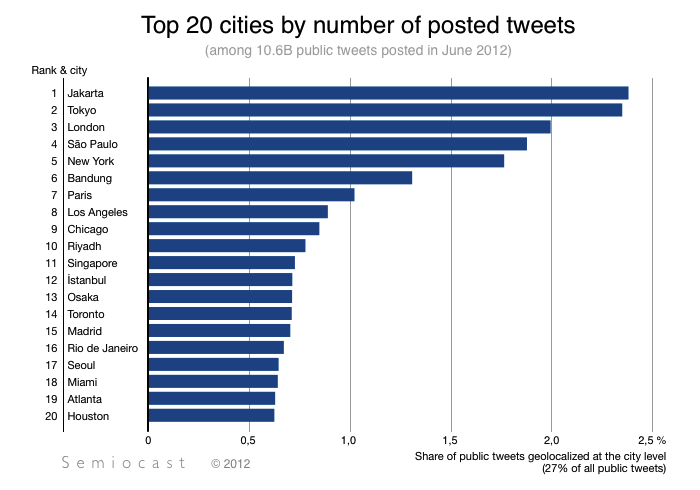
\includegraphics[width=\linewidth]{Gambar/mine/twittercity}
\caption[Top 20 cities by number of posted tweets, dari Semiocast]{Top 20 cities by number of posted tweets, dari Semiocast} 
\label{fig:num_post_tweet}
\end{figure}
Tingginya popularitas Twitter dapat dimanfaatkan untuk berbagai keperluan dalam berbagai aspek. Contohnya sebagai sarana komunikasi, memberikan opini, kampanye poilitik, bisnis, mendapatkan informasi, dan banyak lainya.
\section{Twitter API}
API (Application Programming \textit{interface}) merupakan sebuah cara yang didefinisikan sebuah program untuk menyelesaikan sebuah tugas, biasanya dengan menerima atau memodifikasi data \cite{TwitterApi:2015}. Twitter menyediakan sebuah API yang memberikan hak akses kepada pengembang perangkat lunak untuk membaca dan menulis data dari \textit{server}  Twitter. \textit{Programmer} menggunakan Twitter API untuk membuat aplikasi, \textit{website}, \textit{widgets}, dan proyek lainya yang berinteraksi dengan Twitter. Program akan berkomunikasi dengan Twitter API melalui HTTP. Twitter menyediakan beberapa jenis dan fungsi API yang berbeda, diantaranya REST API, Streaming API, dan ads API.
\subsection{REST API}
REST API menyediakan akses secara program untuk membaca dan menulis data Twitter. Beberapa akses yang disediakan oleh Twitter seperti membuat \textit{tweet} baru, membaca profil \textit{author}, data \textit{follower} dan lain-lain \cite{RESTAPI:2015}. REST API mengidentifikasi aplikasi dan pengguna Twitter menggunakan OAuth. Twitter menyarankan jika pengembang berniat untuk memonitor atau memproses \textit{tweets} secara \textit{real-time} lebih baik menggunakan Streaming API daripada REST API, dikarenakan REST API memiliki \textit{rate limits}.\\\\
\textit{Rate limiting} pada API versi 1.1 ditujukan per-\textit{user} basis atau per \textit{access token}. \textit{Rate limits} pada API versi 1.1 dibagi kedalam selang 15 menit. Ada 2 buah kelompok GET \textit{request} : 15 panggilan setiap 15 menit, dan 180 panggilan setiap 15 menit. Setiap \textit{endpoints} membutuhkan autentikasi. Ini bertujuan agar mencegah kebiasaan yang buruk, dan juga dapat membantu Twitter mengerti lebih jauh bagaimana mengkategorikan aplikasi yang menggunakan API.
\subsection{Streaming API}
Streaming API memberikan latensi yang rendah kepada pengembang untuk mengakses Twitter \textit{global stream} dari data \textit{tweets}. Pengimplementasian secara tepat dan benar dapat menghindari \textit{overhead}. Twitter menawarkan beberapa \textit{streaming endpoints}, setiap \textit{endpoints} telah disesuaikan untuk kasus tertentu \cite{StreamingAPI:2015}.
\begin{enumerate}
	\item \textit{Public Streams}\\
	\textit{Public Stream} menyediakan data publik yang mengalir melewati Twitter. Jenis ini cocok untuk memantau spesifik \textit{user} atau topik, dan penambangan data.
	\item \textit{User Streams}\\
	\textit{User Streams} menyediakan aliran data dan spesifik kejadian untuk \textit{user} yang terautentikasi. \textit{User Streams} tunggal, mengandung semua data yang sesuai dengan \textit{view} yang dimiliki \textit{user} tunggal dari Twitter. 
	\item \textit{Site Streams}\\
	\textit{Site Streams} adalah versi beberapa \textit{user} dari \textit{User Streams}. \textit{Site stream} ditujukan untuk \textit{server}  yang terhubung ke Twitter atas nama banyak \textit{user}. \textit{Site streams} berguna untuk menerima \textit{udates} secara \textit{real-times} dari jumlah \textit{user} yang banyak. 
\end{enumerate}
\subsection{Perbedaaan antara Streaming dan REST}
Streaming API dan REST API memiliki beberapa perbedaan. Karena adanya perbedaan ini, pengembang harus memikirkan jenis API mana yang cocok digunakan dalam aplikasinya. Setiap API memiliki karakteristik dan kelebihan yang berbeda-beda \cite{StreamingAPI:2015}.\\\\
Pada Streaming API, aplikasi memerlukan koneksi HTTP yang tetap terbuka antara \textit{streaming process} dengan \textit{server}  Twitter. Streaming API tidak dapat merespon permintaan \textit{user} secara langsung, namun \textit{user} \textit{request} harus ditangani oleh HTTP \textit{server}  yang dimiliki oleh aplikasi. Pada gambar \ref{fig:stream_api}, aplikasi memiliki 2 buah penanganan yang terdiri dari \textit{server}  yang menangani \textit{user} \textit{request}, dan \textit{server}  yang menangani \textit{streaming process}.\\\\
\begin{figure}
\centering
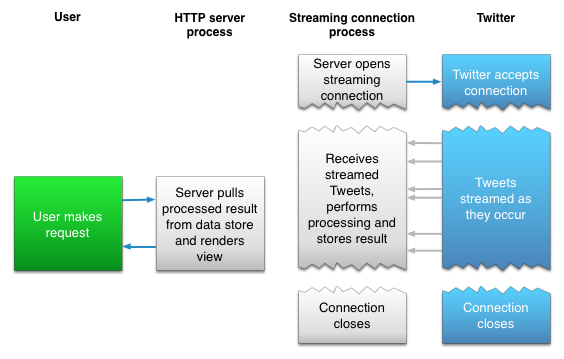
\includegraphics[width=\linewidth]{Gambar/mine/streamingapi}
\caption[Streaming API \textit{Architecture}, dari \cite{StreamingAPI:2015}]{Streaming API \textit{Architecture}, dari \cite{StreamingAPI:2015}} 
\label{fig:stream_api}
\end{figure}
Dalam menggunakan REST API aplikasi idealnya memiliki 2 buah koneksi HTTP. Koneksi \textit{user} dengan HTTP \textit{server}  dan Twitter \textit{server}  dengan HTTP \textit{server}. Permintaan \textit{user} akan diteruskan oleh HTTP \textit{server}  melalui REST API ke \textit{server}  Twitter. Respon dari \textit{server}  Twitter akan diproses oleh HTTP \textit{server}  dan diteruskan kepada \textit{user}. Gambar \ref{fig:rest_api} menggambarkan cara kerja dari REST API.\\
\begin{figure}
\centering
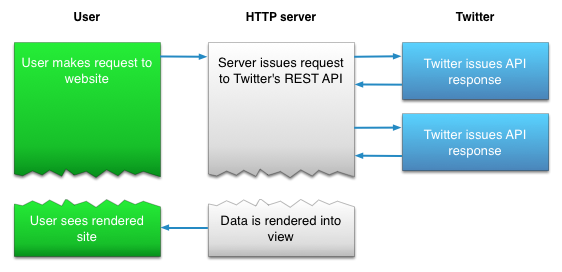
\includegraphics[width=0.8\linewidth]{Gambar/mine/restapi}
\caption[REST API \textit{Architecture}, dari \cite{RESTAPI:2015}]{REST API \textit{Architecture}, dari \cite{RESTAPI:2015}} 
\label{fig:rest_api}
\end{figure}
\section{OAuth}
OAuth 2.0 \textit{authorization} adalah sebuah \textit{framework} yang memungkinkan sebuah aplikasi pihak ke-tiga untuk mendapatkan akses terbatas pada layanan HTTP, tanpa memberikan data autentikasi \cite{RFCOAuth:2012}. Dalam model tradisional autentikasi \textit{client}-server, ketika \textit{client} meminta \textit{requests} sebuah akses terhadap sumber daya yang dilindungi, pemilik dari sumber daya harus memberikan surat kepercayaan kepada \textit{client}. Dalam hal mendukung aplikasi pihak ke-3, pemilik sumber daya harus membagi surat kepercayaanya kepada pihak ke-3. Hal ini menyebabkan beberapa masalah dan batasan : 
\begin{enumerate}
	\item Aplikasi pihak ke-3 perlu menyimpan surat kepercayaan pemilik sumber daya untuk penggunaan dimasa depan, biasanya adalah sebuah textit{password} dalam teks.
	\item \textit{Server}  perlu mendukung autentikasi \textit{password}, walaupun kelemahan keamanan melekat pada \textit{passwords}.
	\item Aplikasi pihak ke-3 mendapatkan seluruh akses pada sumber daya yang dilindungi. Pemilik sumber daya tidak bisa memberikan batasan akses kepada pihak ke-3.
	\item Pemilik sumber daya tidak bisa mencabut akses aplikasi pihak ke-3 tanpa mencabut seluruh akses pihak ke-3, dan harus mengganti password.
\end{enumerate}
OAuth mengatasi masalah ini dengan memperkenalkan sebuah \textit{author}ization \textit{layer} dan membagi peran \textit{client} untuk mengakses sumber daya. Sebagai ganti menggunakan surat kepercayaan pemilik untuk mengakses sumber daya yang dilindungi. \textit{Client} mendapatkan \textit{access token} (sebuah string yang berisi cakupan yang spesifik, waktu akses, dan attribut akses lainya.) \textit{access token} diberikan kepada \textit{client} atau pihak ketiga oleh \textit{author}ization \textit{server}  dengan persetujuan pemiliki sumber daya. \textit{Client} menggunakan \textit{access token} untuk mengakses sumber daya yang dilindungi oleh \textit{resource server}.\\\\
Dalam OAuth didefinisikan ada 4 peran:
\begin{enumerate}
	\item Resource Owner\\
	Sebuah entitas yang dapat memberika akses kepada sumber daya yang dilindungi. Ketika resource owner seorang manusia, ini merujuk pada end-\textit{user}.
	\item Resource Server\\
	\textit{server}  yang menyediakan sumber daya yang dilindungi, dapat menerima dan merespon permintaan sumber daya yang dilindungi menggunakan \textit{access token}s.
	\item \textit{client}\\
	Sebuah aplikasi yang meminta hak akses kepada sumber daya yang dilindungi.
	\item \textit{authorization server}\\
	\textit{server}  yang memberikan \textit{access token}s kepada \textit{client} ketika proses autentikasi berhasil.
\end{enumerate}
\textit{Protocol Flow} dari Oauth akan dijelaskan pada gambar 2.4\\
\begin{figure}
\centering
\includegraphics[width=0.8\linewidth]{Gambar/mine/OAuth}
\caption[\textit{Protocol Flow} Oauth, dari \cite{RFCOAuth:2012}]{\textit{Protocol Flow} Oauth, dari \cite{RFCOAuth:2012}} 
\label{fig:oauth_flow_protocol}
\end{figure}
\begin{enumerate}
	\item \textit{client} melakukan meminta \textit{authorization grant} kepada pemiliki sumber daya. Permintaan bisa dilakukan secara langsung kepada pemilik sumber daya, atau secara tidak langsung melewati \textit{authorization server}  sebagai penengah.
	\item \textit{client} mendapatkan \textit{author}ization grant.
	\item \textit{authorization grant} digunakan untuk meminta \textit{access token} kepada \textit{author}ization Server.
	\item \textit{authorization server}  mengautentikasi apakah \textit{authorization grant} yang dimiliki \textit{client} valid, dan jika valid, \textit{client} diberikan sebuah \textit{access token}.
	\item \textit{client} meminta sumber daya yang dilindungi dari sumber daya \textit{server}  dan melakukan autentikasi dengan memperlihatkan \textit{acces token}.
	\item \textit{resource server}  memvalidasi \textit{access token}, dan jika valid, \textit{server}  akan melayani permintaan.
\end{enumerate}
\section{Twitter4J}
Twitter4j adalah sebuah Java library untuk Twitter API bersifat \textit{open source} dan gratis. Dengan Twitter4j, \textit{user} dapat dengan mudah mengintegrasikan aplikasi Java dengan Twitter service. Twitter4j dapat di unduh pada situs \url{http://twitter4j.org} \cite{Twitter4j:2015}. Berikut beberapa kelas yang dimiliki oleh Twitter4j:\\\\
\textbf{Twitter} adalah sebuah \textit{interface} yang digunakan untuk membungkus Twitter REST API. Method yang dimiliki kelas ini sebagai berikut:
\begin{enumerate}
	\item \textbf{TimelinesResources timelines()}\\
	Berfungsi mendapatkan objek TimelinesResources\\
	\textbf{Kembalian} Mengembalikan sumber daya berupa \textit{timelines} yang dimiliki oleh pemilik sumber daya berdasarkan \textit{access token} Oauth.
	\item \textbf{TweetsResources tweets()}\\
	Berfungsi mendapatkan objek TweetResources\\
	\textbf{Kembalian} Mengembalikan sumber daya berupa \textit{tweets} yang dimiliki oleh pemilik sumber daya berdasarkan \textit{access token} Oauth.
	\item \textbf{SearchResource search()}\\
	Berfungsi mendapatkan objek SearchResource\\
	\textbf{Kembalian} Mengembalikan kelas SearchResource yang dimiliki oleh pemilik sumber daya berdasarkan \textit{access token} Oauth.
\end{enumerate}
\textbf{TwitterFactory} adalah sebuah kelas denggan pattern singleton yang digunakan untuk menginstansiasi kelas Twitter berdasarkan \textit{config tree}. Method yang dimiliki kelas ini sebagai berikut:
\begin{enumerate} 
	\item \textbf{static Twitter getSingleton()}\\
	Berfungsi menginstansiasi kelas Twitter hanya satu kali.\\
	\textbf{Kembalian} instansiasi default singleton Twitter 
\end{enumerate}
\textbf{TwitterStream} adalah sebuah \textit{interface} yang digunakan untuk membungkus Twitter Streaming API. Method yang dimiliki kelas ini sebagai berikut:
\begin{enumerate}
	\item \textbf{void addListener(StreamListener listener)}\\
	Berfungsi menambahkan \textit{listener}.\\
	\textbf{Kembalian} void
	\item \textbf{void removeListener(StreamListener listener)}\\
	Berfungsi menghapus \textit{listener}.\\
	\textbf{Kembalian} void
	\item \textbf{void filter(String query)}\\	
	Berfungsi mengkonsumsi status publik yang sesuai dengan satu atau lebih predikat \textit{filter}.\\
	\textbf{parameter} query - String\\
	\textbf{Kembalian} void
	\item \textbf{void shutdown()}\\
	Berfungsi mematikan thread yang dibagikan oleh instansiasi TwitterStream\\
	\textbf{Kembalian} void
\end{enumerate}
\textbf{TwitterStreamFactory} adalah sebuah kelas yang digunakan untuk menginstansiasi kelas TwitterStream. Method yang dimiliki kelas ini sebagai berikut:
\begin{enumerate}
	\item \textbf{static TwitterStream getSingleton()}\\
	Berfungsi mendapatkan instansiasi dari kelas TwitterStream\\
	\textbf{Kembalian} instansiasi default singleton TwitterStream
\end{enumerate}
\textbf{Paging} adalah sebuah kelas yang digunakan untuk mengontrol \textit{pagination}. Method yang dimiliki kelas ini sebagai berikut:
\begin{enumerate}
	\item \textbf{void setCount(int count)}\\
	Berfungsi untuk mengubah banyaknya status dalam 1 page\\
	\textbf{Parameter} count - int\\
	\textbf{Kembalian} void
	\item \textbf{void setPage(int page)}\\
	Berfungsi untuk mengubah nomor page yang dipilih\\
	\textbf{Parameter} page - int\\
	\textbf{Kembalian} void
\end{enumerate}
\textbf{TimelinesResources} adalah sebuah kelas yang digunakan untuk mengolah timelines berdasarkan hak akses dari \textit{access token}. Method yang dimiliki kelas ini sebagai berikut:
\begin{enumerate}
	\item \textbf{ResponseList<Status> getUserTimeline(String screenName,Paging paging)}\\
	Berfungsi untuk mendapatkan status dari timeline seseorang sejumlah paging yang diinginkan.\\
	\textbf{Parameter} screenName - String, paging - Paging\\
	\textbf{Kembalian} status dari timeline spesifik \textit{user}.
\end{enumerate}
\textbf{SearchResources} adalah sebuah kelas yang digunakan untuk mengolah pencarian berdasarkan hak akses dari \textit{access token}. Method yang dimiliki kelas ini sebagai berikut:
\begin{enumerate}
	\item \textbf{QueryResult search(Query query)}\\
	Berfungsi untuk mendapatkan tweets yang sesuai dengan spesifik query.\\
	\textbf{Parameter} query - Query\\
	\textbf{Kembalian} result dari query diminta
\end{enumerate}
\textbf{Query} adalah sebuah kelas yang digunakan untuk mengolah query untuk menentukan pencarian. Method yang dimiliki kelas ini sebagai berikut:
\begin{enumerate}
	\item \textbf{void setGeoCode(GeoLocation location, double radius, Unit unit}\\
	Berfungsi untuk mencari \textit{tweets} berdasarkan radius tertentu.\\
	\textbf{Parameter} location - GeoLocation, radius - doouble, unit - Query.Unit)\\
	\textbf{Kembalian} void
	\item \textbf{void setLocale(String locale)}\\
	Berfungsi untuk mencari \textit{tweets} hanya pada bahasa tertentu.\\
	\textbf{Parameter} locale - String\\
	\textbf{Kembalian} void
	\item \textbf{void setSince(String since)}\\
	Berfungsi untuk mencari \textit{tweets} sejak tanggal tertentu.\\
	\textbf{Parameter} since - String\\
	\textbf{Kembalian} void
\end{enumerate}
\textbf{Status} adalah sebuah \textit{interface} yang merepresentasikan sebuah status dari seorang \textit{user}. Method yang dimiliki kelas ini sebagai berikut:
\begin{enumerate}
	\item \textbf{java.util.Date getCreatedAt()}\\
	Berfungsi untuk mengetahui tanggal status tersebut dibuat.\\
	\textbf{Kembalian} tanggal status dibuat.
	\item \textbf{long getId()}\\
	Berfungsi untuk mengetahui id status tersebut.\\
	\textbf{Kembalian} id status.
	\item \textbf{java.lang.String getText()}\\
	Berfungsi untuk mengambil isi dari status.\\
	\textbf{Kembalian} isi dari status
	\item \textbf{GeoLocation getGeoLocation()}\\
	Berfungsi untuk mengetahui lokasi tweet bila diketahui.\\
	\textbf{Kembalian} lokasi tweets berasa jika lokasi diketahui.
	\item \textbf{User getUser()}\\
	Berfungsi untuk mengetahui user yang terasosiasi dengan status.\\
	\textbf{Kembalian}user yang terasosiasi dengan status.
\end{enumerate}
\textbf{StatusListener} adalah sebuah \textit{interface} yang merepresentasikan bagaimana status yang dilisten akan ditangani. Method yang dimiliki kelas ini sebagai berikut:
\begin{enumerate}
	\item \textbf{void onDeletion}\\
	Berfungsi menangani ketika \textit{deletionNotices} disampaikan.\\
	\textbf{Kembalian} void.
	\item \textbf{void onStatus}\\
	Berfungsi menangani ketika mendapatkan status ketika melakukan proses \textit{listen}.\\
	\textbf{Kembalian} void.
\end{enumerate}
\section{Jaringan Saraf Tiruan}
Jaringan Saraf Tiruan (JST) adalah paradigma memproses sebuah informasi yang terinspirasi dari cara kerja sistem saraf biologi, seperti otak, memproses informasi \cite{WhatisNN:2015}. Kunci utama dari paradigma ini adalah struktur dari sistem proses informasi. Sistem ini terdiri dari dari banyak unsur proses yang saling terhubung (neuron) bekerja secara serempak untuk menyelesaikan suatu masalah.  JST dikonfigurasi untuk sebuah penerapan yang spesifik, seperti  pengenalan pola atau pengklasifikasian data, melalui proses belajar. Di dalam sistem biologi, belajar melibatkan penyesuaian hubungan sinaptik yang berada diantara neuron.\\\\
Dalam sub bab dibawah peneliti akan membahas beberapa hal mengenai Jaringan Saraf Tiruan meliputi :
\begin{enumerate}
	\item \textbf{Cara Kerja Jaringan Saraf Biologi}, untuk mengerti JST bekerja kita harus mengetahui cara kerja dari jaringan saraf biologi itu sendiri, dalam sub bab ini akan dibahas mengenai jaringan saraf biologi.
	\item \textbf{Masalah yang tidak cocok diselesaikan dengan JST}, dalam sub bab ini akan dibahas bagaimana JST bisa menyelesaikan masalah
	\item \textbf{Masalah yang dapat diselesaikan dengan JST}, dalam sub bab ini akan dibahas jenis permasalahan yang efektif dikerjakan oleh JST
	\item \textbf{Metode Pembelajaran}, agar JST dapat menyelesaikan suatu masalah diperlukan proses belajar seperti halnya jaringan saraf biologi. Bab ini akan membahas metode pembelajaran.
	\item \textbf{Perhitungan Galat}, dalam bab ini akan dibahas cara menghitung galat dari masukan dan keluaran JST.
	\item \textbf{Feedforward Neural Network}, pada bab ini akan dibahas jenis JST yang bernama Feedforward Neural Network.
\end{enumerate}
\subsection{Cara Kerja Jaringan Saraf Biologi}
Untuk membangun sebuah komputer yang dapat berfikir seperti manusia, para
peneiliti harus memodelkanya seperti otak manusia. Komposisi utama otak
manusia adalah sel neuron. JST harus mencoba mensimulasikan sifat-sifat dari
sel neuron itu sendiri.\\\\
Sebuah sel neuron, seperti pada gambar \ref{fig:neuron_biologi}, menerima sinyal dari dendrit. Ketika neuron menerima sebuah sinyal, ada kemungkinan neuron tersebut meneruskan sinyal tersebut. Ketika neuron meneruskanya, sinyal tersebut ditransimisikan melewati axon neuron. Sinyal tersebut akan melewati terminal axon, dan ditransmisikan ke neuron lain.
\begin{figure}
\centering
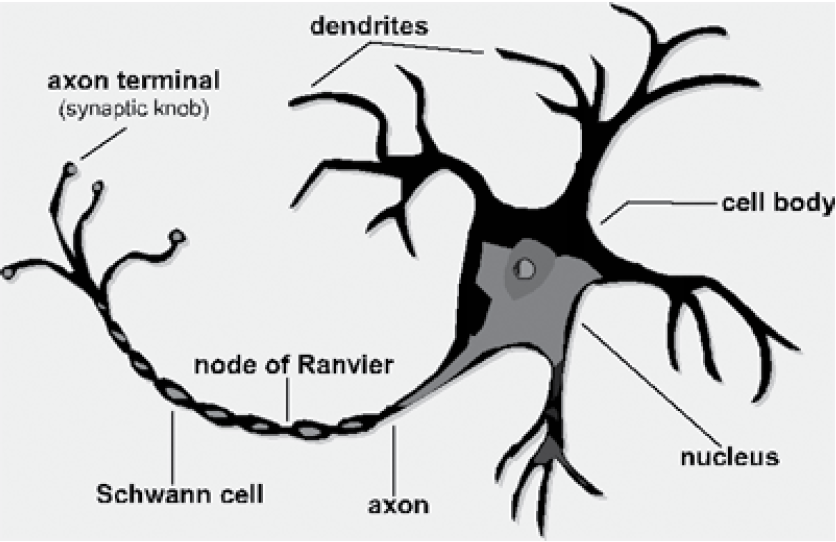
\includegraphics[width=0.7\linewidth]{Gambar/mine/neuron}
\caption[Neuron Biologi, dari \cite{IntroNNforJava:2015}]{Neuron Biologi, dari \cite{IntroNNforJava:2015}} 
\label{fig:neuron_biologi}
\end{figure}
\subsection{Masalah yang tidak cocok diselesaikan dengan JST}
JST dapat memproses kumpulan informasi yang akan menghasilkan keluaran. Keluaran JST nantinya akan digunakan untuk membantu pengambilan sebuah keputusan. Faktanya tidak semua masalah cocok diselesaikan dengan JST. Ada beberapa jenis masalah yang kurang cocok diselesaikan oleh JST :
\begin{enumerate}
	\item Masalah yang dapat diselesaikan dengan program yang mudah untuk di tuliskan kedalam \textit{flowcharts}.
	\item Masalah yang dapat diselesaikan dengan program yang langkahnya dapat didefnisikan dengan terperinci.
	\item Masalah yang harus diketahui cara solusinya diturunkan.
	\item Algoritma yang digunakan untuk menyelesaikan sebuah masalah tidak berubah-rubah (Statik).
\end{enumerate}
\subsection{Masalah yang dapat diselesaikan dengan JST}
Walau tidak semua masalah dapat diselesaikan oleh JST, namun ada banyak hal yang dapat diselesaikan oleh JST. Jenis masalah yang sering diselesaikan oleh JST sebagai berikut :
\begin{enumerate}
	\item \textbf{Classification} adalah proses mengklasifikasian informasi menjadi beberapa
jenis kelompok. Contohnya, perusahaan asuransi ingin mengklasifikasikan permohononan asuransi menjadi beberapa kategori risiko yang berbeda, atau sebuah organisasi online ingin membuat sistem email mereka dapat mengklasifikasikan pesan masuk menjadi kelompok \textit{spam} dan bukan \textit{spam}. Untuk mencapai hal tersebut JST harus dilatih menggunakan beberapa contoh kelompok data dan instruksi. Setiap kelompok data diklasifikasikan menjadi anggota himpunan tertentu. JST dapat belajar dari contoh kelompok data tersebut. Setelah proses pembelajaran diharapkan JST dapat mengindikasi anggota kelompok data yang baru.
	\item \textbf{Prediction} adalah penerapan lain yang sering digunakan untuk JST. Dengan memberikan serangkaian masukan-keluaran data berdasarkan basis waktu, sebuah JST
digunakan untuk memprediksi masa depan. Akurasi prediksi akan bergantung pada banyak faktor, seperti quantiti dan relevansi dari masukan data. JST biasanya diterapkan pada masalah yang melibatkan prediksi pergerakan dalam pasar finansial.
	\item \textbf{Pattern Recognition} adalah sebuah bentuk pengklasifikasian. Pattern recognition adalah kemampuan untuk mengenali pola. Pola harus bisa dikenali bahkan ketika datanya berubah. Sebagai contoh dalam kehidupan kita pengemudi harus dapat dengan tepat mengidentifikasi lampu lalu lintas. Walaupun tidak semua lampu stopan bentuknya sama, pengemudi tetap dapat mengenalinya. Hal ini juga harus dicapai oleh JST agar komputer dapat melakukan pengenalan pola.
	\item \textbf{Pattern Recognition} adalah sebuah bentuk pengklasifikasian. Pattern recognition adalah kemampuan untuk mengenali pola. Pola harus bisa dikenali bahkan ketika datanya berubah. Sebagai contoh dalam kehidupan nyata, pengemudi harus dapat dengan tepat mengidentifikasi lampu lalu lintas. Walaupun tidak semua lampu stopan bentuknya sama, pengemudi tetap dapat mengenalinya. Hal ini juga harus dicapai oleh JST agar komputer dapat melakukan pengenalan pola.
	\item \textbf{Optimization} suatu kemampuan JST untuk mencari solusi yang optimal. Biasanya digunakan ketika suatu masalah memiliki \textit{state space} yang sangat besar. JST mungkin tidak selalu menemukan solusi optimal, namun JST dapat mencari solusi yang dapat diterima. Salah satu masalah optimasi yang paling terkenal ialah Traveling Sales Problem.
\end{enumerate}
\subsection{Metode Pembelajaran}
Ada banyak cara untuk membuat JST dapat belajar. Setiap algoritma pembelajaran nantinya akan melibatkan perubahan bobot setiap penghubung neuron. Proses pelatihan sangatlah penting bagi JST. Ada dua bentuk dari pelatihan yang dapat digunakan,\textit{ supervised }dan \textit{unsupervised}.\textit{ supervised training}melibatkan JST dengan serangkaian masukan-keluaran yang diinginkan. Pada \textit{unsupervised training} dibutuhkan juga kumpulan pelatihan, namun pelatihan tersebut tidak perlu disertai keluaran.
\begin{enumerate}
	\item \textit{Unsupervised training} adalah salah satu metode pembelajaran yang disediakan data masukan namun tidak perlu disediakan antisipasi keluaran. \textit{Unsupervised training} biasanya digunakan untuk melatih JST klasifikasi. Penerapan lainya digunakan untuk data mining. \textit{Unsupervised training} juga biasa digunakan untuk \textit{self-organizing maps} (SOM). \textit{Unsupervised training} dapat diterapkan kedalam banyak situasi. Pada gambar \ref{fig:uns_learning} dijelaskan \textit{flowcharts} proses \textit{unsupervised training}.\\
	
	\begin{figure}
\centering
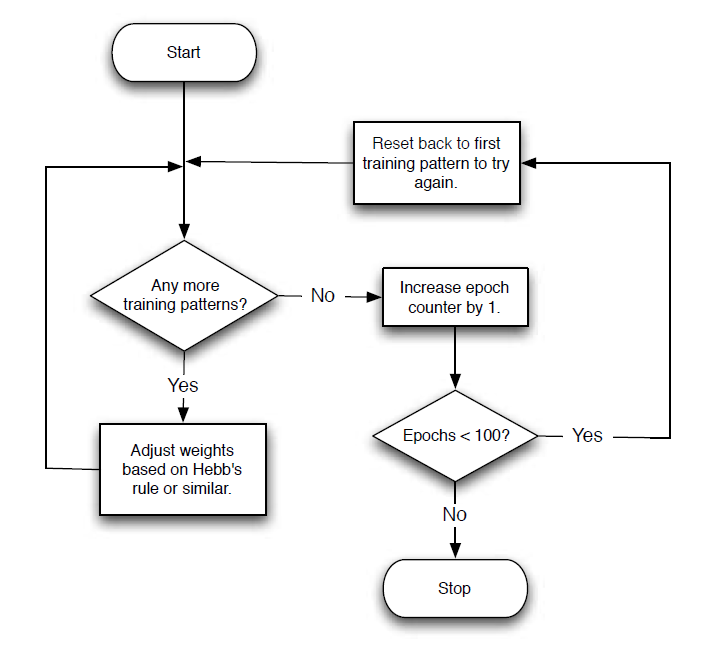
\includegraphics[width=0.8\textwidth]{Gambar/mine/unsupervised}
\caption[\textit{Unsupervised training}, dari \cite{IntroNNforJava:2015}]{\textit{Unsupervised training}, dari \cite{IntroNNforJava:2015}} 
\label{fig:uns_learning}
\end{figure}
	\item \textit{Supervised Training} adalah metode pembelajaran, yang memiliki sekumpulan pelatihan. Perbedaan utama antara\textit{ supervised training} dan \textit{unsupervised training} adalah pada\textit{ supervised training} disediakan harapan keluaran. Hal ini memungkinkan JST untuk menyesuaikan nilai dari bobot matriks  berdasarkan perbedaan antara keluaran yang diharapkan dengan keluaran yang sesunguhnya. Pada gambar \ref{fig:s_learning} dijelaskan \textit{flowcharts} proses \textit{supervised training}.\\\\
	\begin{figure}
	\centering
	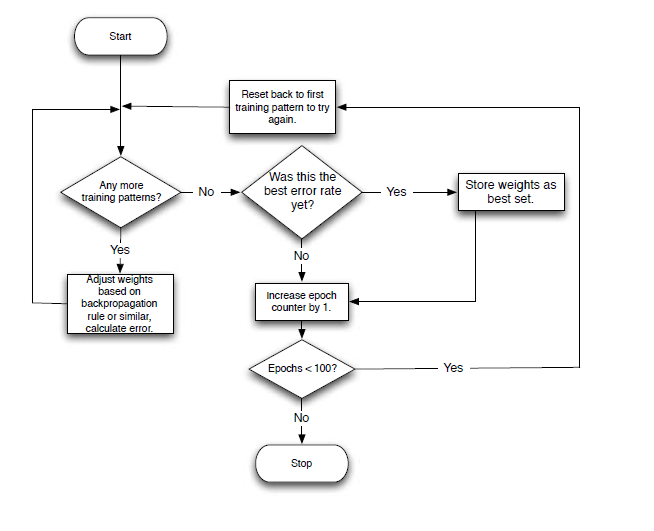
\includegraphics[width=0.8\textwidth]{Gambar/mine/supervised}
	\caption[\textit{Supervised training}, dari \cite{IntroNNforJava:2015}]{\textit{Supervised training}, dari \cite{IntroNNforJava:2015}} 
	\label{fig:s_learning}
	\end{figure}
\end{enumerate}
\subsection{Perhitungan Galat}
Perhitungan galat adalah salah satu aspek penting dari setiap pelatihan JST. Apakah pelatihan itu adalah\textit{ supervised }atau \textit{unsupervised}, sebuah rata-rata galat harus dihitung. Tujuan dari setiap algoritma pelatihan ialah untuk meminimalisasi rata-rata galat.
\subsubsection{Perhitungan Galat dan\textit{ supervised }Training}
Ada dua nilai yang harus dipertimbangkan dalam menentukan rata-rata galat untuk\textit{ supervised training}. Pertama kita harus menghitung galat untuk setiap element pelatihan. Kedua, kita harus menghitung rata-rata galat untuk semua element pelatihan untuk setiap sampel. (Root Mean Square) RMS adalah salah satu metode untuk menghitung rata-rata galat untuk sebuah pelatihan. Metode RMS efektif dalam perhitungan rata-rata galat, tanpa memperhatikan apakah hasil yang sebenarnya lebih tinggi atau lebih kecil daripada hasil yang diharapkan. Untuk menghitung RMS digunakan formula. 
\begin{displaymath}
	x_{rms}= \sqrt{\frac{1}{n}\sum_{i=1}^{n}(aktual_{i}-ideal_{i})^2}	
\end{displaymath}
Dimana n adalah jumlah pasangan masukan dan keluaran, aktual adalah keluaran yang dihasilkan oleh JST, dan ideal adalah keluaran yang diinginkan. Dengan mengetahui rata-rata galat dari keluaran yang diharapkan dan yang sebenarnya, kita dapat menentukan apakah JST tersebut sudah cukup baik atau belum.
\subsection{Feedforward Neural Network}
Feedforward adalah sebuah arsitektur JST yang populer dan banyak digunakan sebagai model dalam banyak penerapan. Feedforward dikenal juga sebagai ``multi-layer perceptron''. Dalam JST feedforward, setiap layer dari JST mengandung hubungan ke layer berikutnya (contohnya dari layer masukan dihubungkan ke layer tersembunyi) ilustrasi feedforward pada gambar \ref{fig:ffnn}. Hubungan antar neuron pada feedforward hanya satu arah. Feedfoward selalu dimulai dari layer masukan. Jika masukan terhubung dengan sebuah layer tersembunyi, layer tersembunyi dapat terhubung dengan layer tersembunyi lainya atau dapat langsung terhubung dengan layer keluaran. Jumlah layer tersembunyi bisa banyak. Kebanyakan JST biasanya akan memiliki satu buah layer tersembunyi, dan akan sangat jarang JST memiliki lebih dari dua buah layer tersembunyi.\\
\begin{figure}
	\centering
	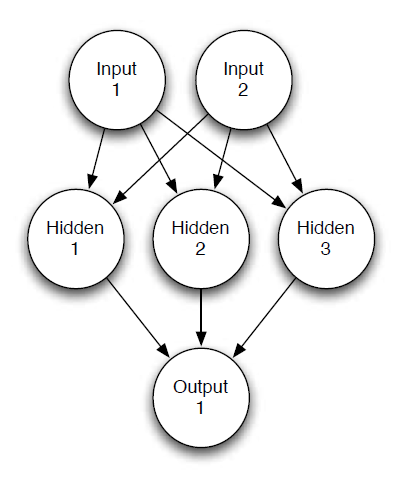
\includegraphics[width=0.6\linewidth]{Gambar/mine/ffnn}
	\caption[Contoh Feed Forward Neural Network, dari \cite{IntroNNforJava:2015}]{Contoh Feed Forward Neural Network, dari \cite{IntroNNforJava:2015}} 
	\label{fig:ffnn}
	\end{figure}
\textbf{Memilih Struktur Jaringan}\\
Ada banyak cara untuk membangun JST feedforward. Kita harus menentukan berapa jumlah neuron pada layer masukan dan layer keluaran. Selain itu layer tersembunyi harus ditentukan. Ada banyak teknik untuk memilih parameter tersebut. Untuk menentukan struktur yang optimal pada feedforward dibutuhkan pengalaman dan percobaan.
\begin{enumerate}
\item\textbf{Layer masukan}\\Jumlah neuron pada layer masukan dapat ditentukan bergantung pada data yang kita miliki. Parameter ini biasanya ditentukan secara unik ketika kita mengetahui data pelatihan kita. Secara spesifik, jumlah dari neuron setara dengan banyaknya kolum pada data kita. Biasanya kita dapat menambahkan satu buah titik bias.
\item\textbf{Layer Keluaran}\\Seperti layer masukan, setiap JST memiliki satu buah layer keluaran. Untuk jumlah neuron di dalamanya ditentukan pada model apa yang kita gunakan. Apakah JST kita \textit{Machine Mode} atau \textit{Regression Mode}. Jika pada \textit{Machine Mode} JST akan mengembalikan kelas, sedangkan pada \textit{Regression Mode} mengembalikan sebuah nilai. bila JST menggunakan sebuah regressor, maka keluarannya akan memiliki 1 neuron. Bila keluarannya sebuah pengklasifikasian, maka akan memiliki satu neuron atau lebih.
\item\textbf{Layer Tersembunyi}\\Dalam menentukan layer tersembunyi ada dua buah keputusan yang harus diperhatikan. Pertama menentukan berapa jumlah layer tersembunyi yang dibutuhkan. Kedua menentukan berapa jumlah neuron pada setiap layer.\\\\ 
Secara teori tidak ada alasan untuk menggunakan layer tersembunyi lebih dari dua. Faktanya pada masalah yang ada pada kehidupan sehari-hari, dengan 1 buah layer tersembunyi banyak masalah dapat diselesaikan. Tabel \ref{table:jmlhHiddenLayer} merupakan kegunaan JST berdasarkan banyaknya layer tersembunyi\\\\
\begin{table}
\centering
\caption{Menentukan jumlah hidden layer}
\label{table:jmlhHiddenLayer}
\begin{tabular}{|l|p{12cm}|}
\hline
Jumlah Hidden Layer & Kegunaan \\\hline
tidak ada & Hanya dapat merepresentasikan fungsi linear atau pemilihan linear.\\\hline
1 & Dapat memeperikaran semua fungsi yang mengandung pemetaan kontinu dari satu \textit{space} terbatas ke yang lainya.\\\hline
2 & Dapat merepresentasikan sebuah keputusan yang  batasanya dan akurasi yang berubah-ubah dengan fungsi aktivasi rasional dan dapat memperkirakan setiap pemetaan halus untuk akurasi apapun.\\\hline
\end{tabular}
\end{table}
Untuk menentukan jumlah neuron dalam layer tersembunyi adalah bagian yang sangat penting dalam menentukan keseluruhan arsitektur JST. Walaupun layer ini tidak secara langsung berinteraksi dengan lingkungan luar, layer ini memiliki pengaruh yang sangat besar pada akhir keluaran. Jumlah layer tersembunyi dan jumlah neuronya sangat penting diperhatikan. Jika kita terlalu sedikit menggunakan neuron dalam layer tersembunyi ini akan mengakibatkan sesuatu yang disebut \textit{underfitting}. Namun bila terlalu banyak menggunakan neuron pada layer tersembunyi ini akan mengakibatkan \textit{overfitting}. \textit{Overfitting} terjadi ketika JST terlalu banyak memiliki informasi yang diproses daripada jumlah batas dari informasi yang terkandung dalam sejumlah pelatihan. Ada beberapa tips untuk menentukan jumlah neuron: Pertama jumlah neuron harus berada diantara jumlah masukan dan keluaran. Kedua jumlah neuron seharusnya 2/3 ukuran dari layer masukan, ditambah dengan layer keluaran. Ketiga jumlah neuron seharusnya kurang dari dua kali dari layer masukan.
\item\textbf{Fungsi Aktivasi}\\
Kebanyakakn JST mengeluarkan keluaran dari layernya menggunakan fungsi aktivasi. Fungsi aktivasi ini menskalakan keluaran dari JST dalam jangkauan tertentu. Fungsi aktivasi dapat kita buat sendiri namun umumnya menggunakan fungsi yang sudah sering digunakan. Ada beberapa jenis fungsi aktivasi yang sering digunakan diantara sebagai berikut:\\\\
\textbf{Sigmoid} adalah fungsi aktivasi yang menggunakan fungsi sigmoid untuk menentukan aktivasi. fungsi sigmoid di definisikan sebagai berikut:
\begin{displaymath}
	f(x)=\frac{1}{1+e^{-x}}
\end{displaymath}
Kurva \ref{fig:k_sigmoid} menggambarkan fungsi sigmoid. Dalam perhitungan sigmoid berapapun parameter x maka y tidak akan lebih dari satu dan kurang dari nol
\begin{figure}
	\centering
	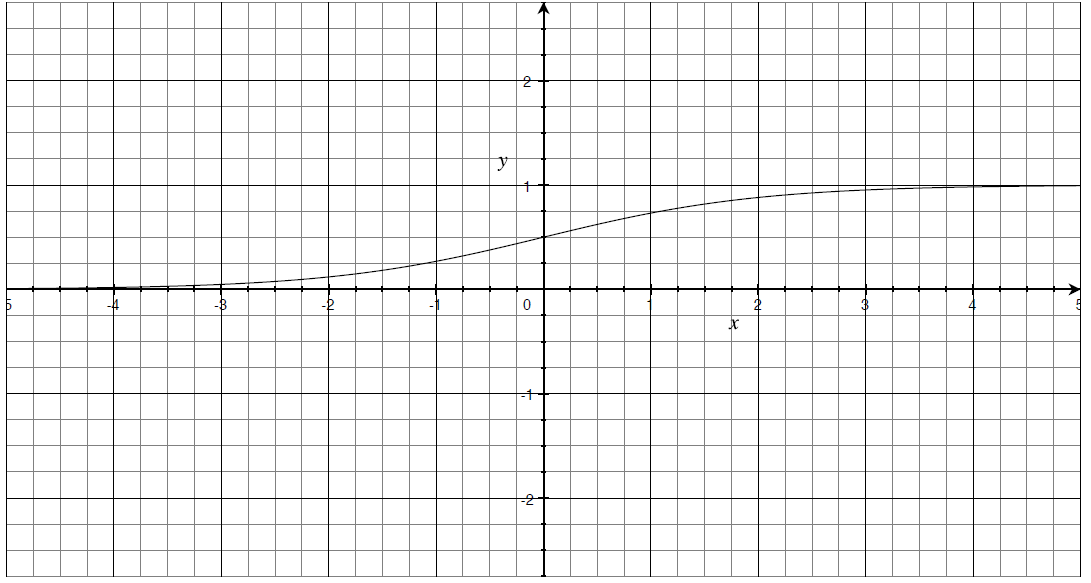
\includegraphics[width=0.6\linewidth]{Gambar/mine/sigmoid}
	\caption[Kurva Sigmoid, dari \cite{IntroNNforJava:2015}]{Kurva Sigmoid, dari \cite{IntroNNforJava:2015}} 
	\label{fig:k_sigmoid}
	\end{figure}
Hal penting yang perlu diperhatikan dalam menggunakan fungsi sigmoid. Fungsi ini hanya akan menghasilkan nilai positif.\\\\
\textbf{Hyperbolic Tangent}
Jika pada fungsi sigmoid y akan selalu selalu bernilai positif. Dengan menggunakan fungsi Hyperbolic Tangent maka nilai y bisa bernilai negatif. Jika keluaran yang kita ingin dapat bernilai negatif dan positif, kita dapat menggunakan fungsi Hyperbolic Tangent yang di definisikan sebagai berikut:
\begin{displaymath}
	f(x)=\frac{e^{2x}-1}{e^{2x}+1}
\end{displaymath}
Kurva \ref{fig:k_tangent} menggambarkan fungsi Hyperbolic Tangent dimana nilai y dapat bernilai positif atau negatif bergantung pada x yang diberikan.
\begin{figure}
	\centering
	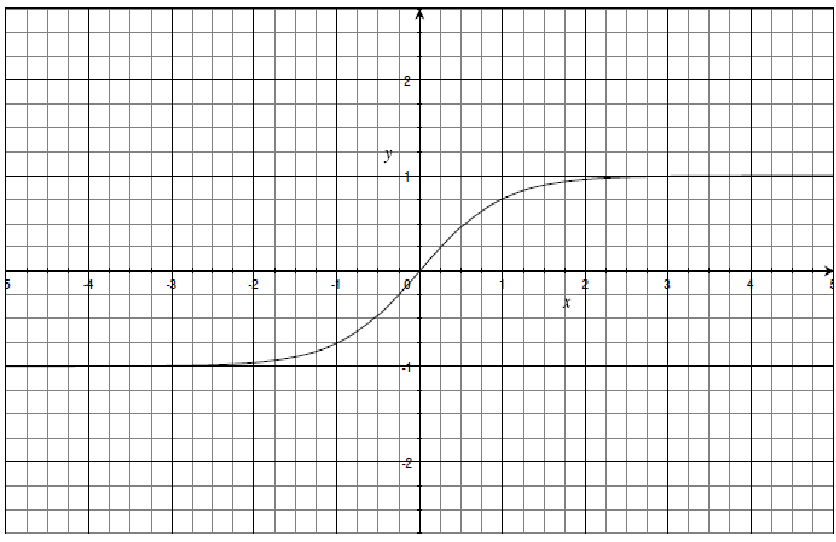
\includegraphics[width=0.6\linewidth]{Gambar/mine/tangent}
	\caption[Kurva Tangent, dari \cite{IntroNNforJava:2015}]{Kurva Tangent, dari \cite{IntroNNforJava:2015}} 
	\label{fig:k_tangent}
	\end{figure}
\end{enumerate}
\subsection{Backpropagation}
\textit{Backpropagation} adalah salah satu metode untuk melakukan pelatihan pada jaringan feedforward yang memiliki beberapa layer. \textit{Backpropagation} dapat digunakan untuk setiap jaringan feedforward yang menggunakan sebuah fungsi aktivasi yang dapat diturunkan. Pada backpropagation bobot setiap penghubung antar neuron akan dirubah agar JST dapat menghasilkan keluaran yang diharapkan sesedikit mungkin mengalami kesalahan.\\\\ 
\section{Database Management System}
\subsection{Fungsi dan karakteristik DBMS}
Secara tradisional pengorganisasian data biasanya dalam format file. Karena banyak kekurangan yang dimiliki dari pengorgansiasian tradisional (format file), maka dirancanglah sebuah konsep baru bernama Database Managment System (DBMS) untuk menutupi kekurangan penyimpanan tradisional \cite{DBMS:2015}.  Pada DBMS modern memiliki karakteristik sebagai berikut :
\begin{enumerate}
	\item \textbf{Real-world entity} : DBMS modern dirancang agar lebih realistik dengan menggunakan entitas yang berada di dunia nyata untuk merancang arsitekturnya. DBMS juga memiliki atribut dan kebiasaan dari entitas itu sendiri.
	\item \textbf{Relation-based tables} : DBMS memperbolehkan hubungan antar entitas kedalam bentuk tabel. Dengan hal tersebut pengguna dapat mengerti arsitektur dari basis data hanya dengan  melihat nama-nama tabelnya.
	\item \textbf{Isolation of data and application} : Sistem basis data seluruhnya berbeda dari datanya. Sebuah basis data adalah sebuah entitas aktif, sedangkan datanya adalah entitas pasif. DBMS menyediakan metadata, yaitu data mengenai data.
	\item \textbf{Less redundancy} : DBMS mengikuti peraturan normalisasi, dimana membagi sebuah relasi ketika atribut unik dari entitas tersebut memiliki nilai yang sama.
	\item \textbf{Consistency} : Konsistensi adalah status dimana setiap relasi dalam basis data tetap sesuai dengan yang seharusnya (tidak terjadi perubahan yang membingungkan). Pada DBMS ada beberapa metode dan teknik, yang dapat mendeteksi ketidak konsistenan data. 
	\item \textbf{Query Language} : DBMS diperlengkapi dengan bahasa query, yang membuat DBMS lebih efisien ketika ingin mendapatkan dan memanipulasi data.  
	\item \textbf{ACID Properties} : DBMS menerapkan perinsip \textbf{A}tomicity, \textbf{C}onsitency, \textbf{I}solation, \textbf{D}urabillity (Disingkat ACID). Dengan menerapkan prinsip ACID, membantu basis data tetap sehat dalam menangani banyak transaksi data. 
	\item \textbf{Concurrent Access} : DBMS mendukung multi-user dalam mengakses dan memanipulasi data dalam waktu yang bersamaan.
	\item \textbf{Security} : DBMS menawarkan banyak perbedaan level keamanan. Hal ini dapat membatasi setiap user dalam mengakses dan memanipulasi data.
\end{enumerate} 
\subsection{Data Model}
Data model mendefinisikan bagaimana struktur logika dari basis data di modelkan. Data model juga mendefinisikan bagaimana setiap data terhubung dengan yang lain dan bagaimana data diproses dan disimpan didalam sistem \cite{DBMS:2015}. Data model yang pertama kali digunakan adalah flat data-model, dimana semua data yang digunakan disimpan didalam tempat yang sama dan menyebabkan banyak duplikasi dan pembaruan yang anomali. Karena banyak kelemahan yang dimiliki flat data-model makan dirancang data model yang diharapkan lebih baik diantaranya :\\\\
\textbf{Entity-Relationship Model}\\
Entity-Relationship (ER) Model diciptakan berdasarkan karakteristik DBMS dari Real-World Entities dan hubungan antar entitasnya. Untuk memodelkan Real-World Entites kedalam DBMS dibutukah sebuah model konseptual, maka digunakanlah ER Model. Pada gambar \ref{fig:erd} menunjukan konsep ER Model.
	\begin{figure}
	\centering
	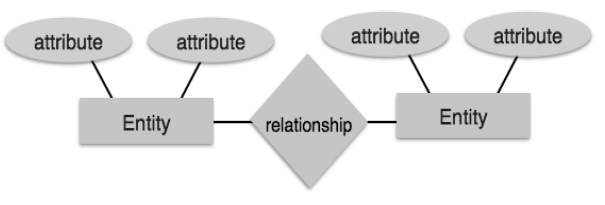
\includegraphics[width=0.6\linewidth]{Gambar/mine/erd}
	\caption[ER Model, dari \cite{DBMS:2015}]{ER Model, dari \cite{DBMS:2015}} 
	\label{fig:erd}
	\end{figure}
\begin{enumerate}
	\item \textbf{Entity}\\
	\textit{Entity} atau entitas dalam ER Model adalah sebuah entitas di dunia nyata yang memiliki sifat disebut \textbf{attribute} atau atribut. Setiap atribut di definisikan oleh sekumpulan nilai yang disebut \textbf{domain}.
	\item \textbf{Relationship}\\
	Asosiasi logika antar entitas disebut \textbf{relationship}. Relationship dipetakan dengan entitas dengan cara yang bervariasi. Untuk memetakan kardinalitas antar entitas dapat didefinisikan dengan angka dari asosiasi diantara kedua entitas. Jenis pemetaan kardinalitas diantaranya \textit{one to one, one to many, many to one, many to many}.
\end{enumerate}
\textbf{Relational Model}\\
Relational model adalah pengorganisasian data kedalam sekumpulan tabel yang datanya dapat di akses atau dirakit kembali kedalam banyak cara tanpa harus melakukan organisasikan kembali pada tabel database Gambar \ref{fig:relational} menunjukan contoh relational model \cite{RelationDefinition:2001}. Setiap table (atau kadang disebut relasi) mengandung satu atau lebih kategori data dalam kolom (\textit{attribute}). Setiap baris (\textit{tuples}) mengandung instansiasi yang unik dari data. Keuntungan menggunakan relational model daripada model lainya :
\begin{enumerate}
	\item Berdasarkan pengertian matematika relasi dan himpunan, sehingga dapat menggunakan abstraksi matematika.
	\item Menggunakan struktur data yang sederhana, mudah dimengerti.
	\item Membagi level logis dan level fisikal. 
	\item Operasi tidak perlu mengerti struktur data yang digunakan.
\end{enumerate}
	\begin{figure}
	\centering
	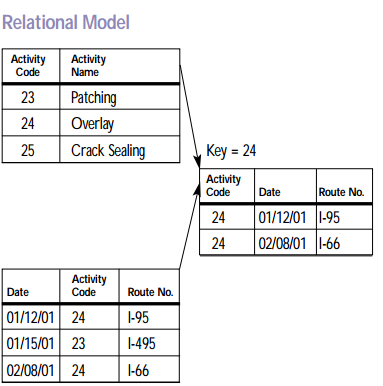
\includegraphics[width=0.6\linewidth]{Gambar/mine/relational}
	\caption[Model Relational, dari \cite{RelationDefinition:2001}]{Model Relational, dari \cite{RelationDefinition:2001}} 
	\label{fig:relational}
	\end{figure}
\subsection{SQL}
SQL kepanjangan dari Structured Query Language adalah sebuah bahasa standard untuk mengakses dan memanipulasi basis data. SQL adalah sebuah standard ANSI(American National Standards Institute). Dengan menggunakan \textit{statement} SQL kita dapat memanipulasi sebuah basis data. Setiap \textit{statement} memiliki sintaksis. Berikut beberapa sintaksis dasar dan fungsinya :
\begin{enumerate}
	\item SELECT columnNname, columnNname FROM tableName WHERE columnName operator value \\ Berfungsi mengambil data berdasarkan kolom dari sebuah Tabel dengan kondisi dimana nilai dari column tersebut memenuhi suatu nilai.
	\item INSERT INTO tableName VALUES value1,value2,value3,...\\
Berfungsi memasukan nilai-nilai kedalam sebuah table atau relasi.
	\item UPDATE tableName SET column1=value1,column2=value2,... WHERE someColumn=someValue\\
Berfungsi merubah nilai-nilai pada sebuah table di sebuah \textit{tuple} yang memenuhi sebuah kriteria
	\item DELETE FROM tableName WHERE someColumn=someValue\\
	Berfungsi menghapus sebuah \textit{tuple} yang memiliki kriteria tertentu
\end{enumerate}
\subsection{MySQL}
MySQL adalah salah satu Relational DBMS \textit{open source} yang paling populer di dunia. MySQL dapat membantu pengembang mendapatkan aplikasi basis data yang memiliki performa tinggi, \textit{scalable} dan \textit{cost-effectively}. MySQL menyediakan edisi gratis dan komersial. Edisi Gratis MySQL dapat diunduh bersama Apache dan PHP dalam paket XAMPP di situs \url{https://www.apachefriends.org/index.html}.
\subsection{JDBC}
JDBC adalah sebuah API yang di rancang untuk menghubungkan basis data SQL dengan pemograman berbahasa Java. JDBC menyediakan metode untuk melakukan \textit{query} dan \textit{updating} data kedalam database. JDBC berorientasi dengan basis data relasional. Berikut beberapa kelas yang dimiliki oleh JDBC:\\
\textbf{Connection} adalah sebuah interface yang berfungsi melakukan koneksi dengan sebuah spesifik basis data. Method yang dimiliki kelas ini sebagai berikut:
\begin{enumerate}
	\item \textbf{Statement createStatement()}\\
	Berfungsi membuat sebuah objek Statement untuk mengirimkan SQL statments kedalam basis data.\\
	\textbf{Kembalian} Statement
	\item prepareStatement(String sql)
	Berfungsi membuat objek PrepareStatement untuk mengirimkan parameter SQL kedalam database.\\
	\textbf{Parameter} sql - String
	\textbf{Kembalian} sebuah objek PreparedStatement
\end{enumerate}
\textbf{DriverManager} Layanan dasar untuk mengelola satu set JDBC driver. Method yang dimiliki kelas ini sebagai berikut:
\begin{enumerate}
	\item \textbf{Connection getConnection(String url)}\\
	Berfungsi mendapatkan objek Connection
	\textbf{Parameter} url - String\\
	\textbf{Kembalian} objek Connection
\end{enumerate}
\textbf{PreparedStatement} Adalah sebuah kelas yang merepresentasikan sebuah \textit{precomplied SQL statment}. Method yang dimiliki kelas ini sebagai berikut:
\begin{enumerate}
\item \textbf{void Execute()}
Berfungsi melakukan eksekusi terhadap query
\textbf{Kembalian} void
\end{enumerate}
\textbf{Statement} Adalah sebuah interface yang berfungsi mengeksekusi perintah SQL statik dan mengembalikan hasil perintah tersebut. Method yang dimiliki kelas ini sebagai berikut:
\begin{enumerate}
	\item \textbf{ResultSet executeQuery(String sql)}\\
	Berfungsi mengeksekusi perintah SQL yang diberikan.\\
	\textbf{Parameter} sql - String
	\textbf{Kembalian} sebuah objek ResultSet
\end{enumerate}}{}
\ifdefstring{\vbabc}{1}{\chapter{Analisis}
\section{Arsitektur Perangkat Lunak}
Pada penelitian ilmiah ini akan dibangun sebuah perangkat lunak yang bertujuan membantu penggunanya untuk memprediksi kemacetan di kota Bandung. Perangkat lunak ini terdiri dari 3 lapisan utama: Lapisan pertama berfungsi mendengarkan \textit{tweets} yang telah disaring dan berasal dari Twitter \textit{streaming}. Lapisan kedua adalah pra-proses data agar \textit{tweets} yang telah disaring dirubah menjadi bahan pembelajaran JST yang terstruktur dengan baik, pada lapisan ini dibutuhkan interaksi manusia. Pada lapisan ketiga dalam perangkat lunak ini berfungsi memprediksi kemacetan berdasarkan nama jalan dan waktu. Arsitekturnya dapat dilihat pada gambar \ref{fig:arsitekturpl}
\begin{figure}
\centering
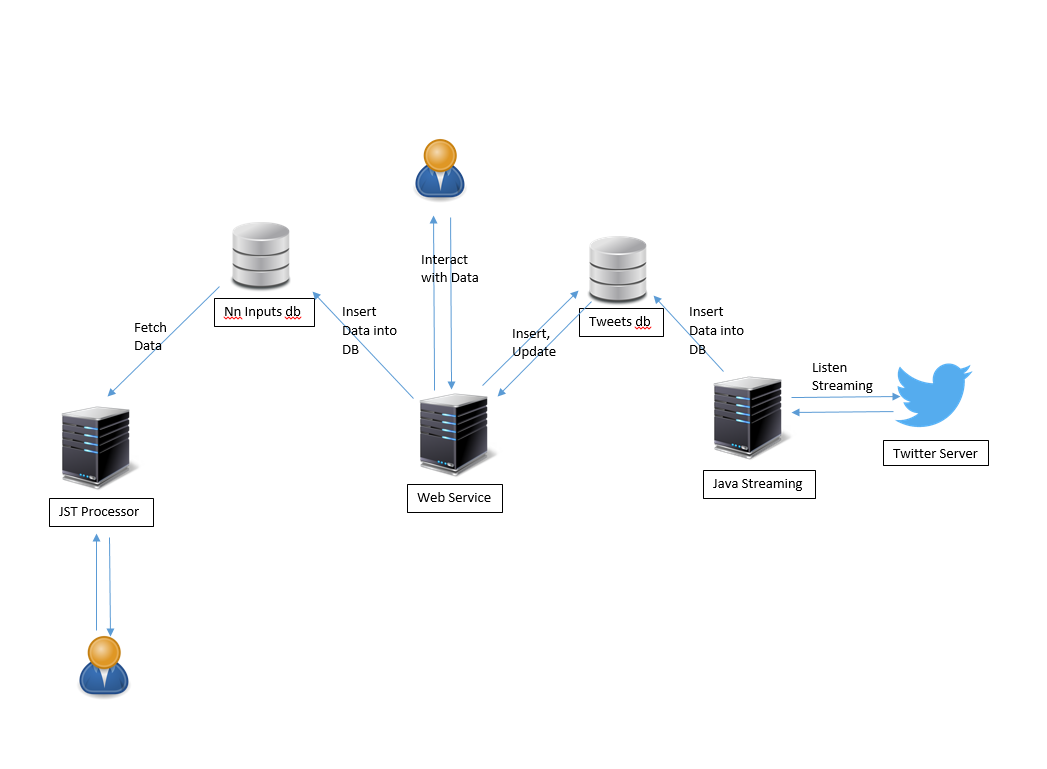
\includegraphics[width=0.6\linewidth]{Gambar/mine/sistem}
\caption[Arsitektur Perangkat Lunak]{Arsitektur Perangkat Lunak} 
\label{fig:arsitekturpl}
\end{figure}
\section{REST API atau Streaming API}
Pada lapisan pertama arsitektur digunakan untuk menarik \textit{tweets} yang berasal dari Twitter. Untuk menarik \textit{tweets} dari Twitter kedalam perangkat lunak akan digunakan \textit{library} Java bernama Twitter4j, library ini telah membungkus Twitter API agar dapat diimplementasikan kedalam pemograman bahasa Java. Pada bab dasar teori membahas bahwa Twitter API memiliki 2 cara dalam penarikan data yaitu REST API dan Streaming API. Bila kita teliti pada kebutuhan perangkat lunak, diperlukan jumlah data yang tidak sedikit untuk melakukan pemrosesan data pada arsitektur lapisan ketiga, maka harus dipilih jenis Twitter API yang dapat mengambil data secara berkala. Jika kita melihat salah satu API Twitter, REST API memiliki \textit{rate limits} yang membatasi perangkat lunak hanya dapat memanggil 180 perintah setiap 15 menit, karena batasan ini ada kemungkinan \textit{tweets} yang berharga dapat terlewat bahkan terjadi duplikasi \textit{tweets}. Berbeda seperti REST API, Streaming API tidak memiliki batasan untuk melakukan \textit{listen} pada server Twitter, dengan hal ini dapat memudahkan perangkat lunak dalam mengambil \textit{tweets} yang berlalu lalang di Server Twitter. Oleh karena itu perangkat lunak akan menggunakan Streaming API yang telah dibungkus oleh Twitter4j.
\section{Jenis Jaringan Syaraf Tiruan}
Tujuan penelitian ini adalah membangun perangkat lunak yang dapat memprediksi kemacetan. Jaringan Syaraf Tiruan adalah salah satu teknik yang tepat untuk memprediksi suatu kejadian berdasarkan kejadian-kejadian yang terjadi sebelumnya. Salah satu jenis JST yang popular dan sering digunakan untuk memprediksi ialah \textit{Feed Forward}. Untuk menggunakan JST \textit{Feed Foward} ada beberapa hal yang perlu ditentukan agar JST \textit{Feed Foward} dapat bekerja secara optimal, hal yang perlu ditentukan antar lain :
\begin{enumerate}
	\item Jumlah Hidden Layer dan Neuron setiap \textit{layer}
	\item Fungsi Aktivasi
	\item Metode Pembelajaran JST
\end{enumerate}
\subsection{Jumlah Hidden Layer dan Neuron setiap \textit{layer}}
Pada JST \textit{Feed Forward} terdiri 3 jenis \textit{layer}, \textit{input layer}, \textit{hidden layer}, \textit{output layer}. Setiap \textit{layer} terdiri dari neuron-neuron. Jumlah neuron ini perlu ditentukan,hal ini bergantung pada masalah dan keperluan JST. Dalam sub-bab ini peneliti akan menganalisis jumlah neuron setiap \textit{layer}-nya berdasarkan teknik yang telah dipaparkan pada bab-2. \\
Sebelum menentukan jumlah neuron setiap \textit{layer} pertama yang akan kita akan menentukan jumlah \textit{hidden layer}. Jumlah \textit{hidden layer} akan menentukan fungsi dari JST itu sendiri. Kita dapat melihat kembali pada tabel \ref{table:jmlhHiddenLayer} untuk menentukan jumlah hidden layer berdasarkan kegunaanya. Dapat hal memprediksi kemacetan dapat dimodelkan sebagai fungsi yang mengandung pemetaan kontinu. Oleh karena itu dengan hanya menggunakan satu buah hidden layer sudah cukup agar JST dapat memodelkan fungsi prediksi kemacetan.\\\\
Setelah menentukan jumlah \textit{hidden layer} kita akan menentukan jumlah neuron dalam \textit{input neuron}. Jumlah neuron pada \textit{input layer} bergantung pada data yang kita miliki, dan parameter apa saja yang diperlukan untuk melatih JST. Jika kita meninjau struktur data pelatihan terdiri dari hari, jam, nama lokasi, dan status kemacetan. Oleh karena itu jumlah neuron dalam \textit{hidden layer} akan berjumlah 4 buah.\\\\
Sama seperti \textit{input layer}, \textit{output layer} ditentukan berdasarkan kebutuhan. Karena \textit{output layer} berfungsi menentukan output tersebut berstatus macet atau tidak, makan jumlah neuron dalam output layer akan memiliki 2 buah neuron. Dimana setiap neuron akan merepresentasikan status dari kemacetan.\\\\
Berbeda dengan menentukan \textit{input} dan textit{output layer} tidak ada cara baku untuk menentukan jumlah \textit{hidden layer} namun ada teknik-teknik yang membantu kita menentukan jumlah \textit{hidden layer}. Pada bab-2 telah dipaparkan jumlah neuron harus berada diantara jumlah masukan dan keluaran. Jumlah neuron seharusnya 2/3 ukuran dari layer masukan, ditambah dengan layer keluaran. Ketiga jumlah neuron seharusnya kurang dari dua kali dari layer masukan. Bila menggunakan teknik tersebut jumlah neuron pada \textit{hidden layer} berjumlah 4 neuron.
\subsection{Fungsi Aktivasi}
Dalam bab-2 dipaparkan bahwa fungsi aktivasi dapat kita buat dan tentukan berdasarkan kebutuhan. Namun keluaran yang dihasilkan JST hanya akan menentukan apakah prediksi tersebut macet atau tidak, \textit{range} angka nol sampai satu sudah dapat merepresentasikan apakah keluaran bernilai macet atau tidak. Karena \textit{range}nya bernilai nol sampai satu, kita dapat menggunakan fungsi aktivasi yang sering digunakan yaitu sigmoid. Fungsi aktivasi sigmoid hanya akan menghasilkan nilai nol sampai dengan satu dapat kita lihat pada gambar \ref{fig:k_sigmoid} pemetaan fungsi sigmoid.
\subsection{Metode Pembelajaran}
\section{Pengumpulan data pelatihan JST}
Agar JST dapat memprediksi kemacetan dengan tepat, maka JST perlu dilatih dilakukan pembelajaran. Karena JST perlu belajar maka dibutuhkanya kumpulan data pelatihan. Data yang digunakan untuk memprediksi ialah data kejadian yang pernah terjadi di masa lalu. Data pelatihan ialah \textit{tweets} yang bersumber dari media sosial Twitter yang akan diambil oleh sistem secara kontinu. \textit{Tweets} yang akan dijadikan metode pelatihan akan disaring berdasarkan \textit{query} tertentu. Kriteria dibawah akan menjadi penyaring jenis \textit{tweets} apa yang akan diambil sebagai pra-data pelatihan.
\begin{enumerate}
	\item Pemilihan Nama Jalan
	\item Pemilihan Sumber \textit{tweets}
	\item Bahasa
\end{enumerate}
\subsection{Pra-proses input JST}
Setelah kita melakukan penyaringan terhadap \textit{tweets}, agar menjadi data pelatihan bagi JST kita harus melakukan pra-proses agar \textit{tweets} menjadi masukan yang dapat diterima bagi JST. Cara yang kita gunakan memprosesnya dengan cara manual yang menggunakan manusia untuk memparsing \textit{tweets} menjadi input JST. Pertama manusia akan memilih apakah \textit{tweets} memenuhi kriteria sebagai input JST. Kedua \textit{tweets} yang memenuhi kriteria akan di pra-proses informasi apa yang terdapat dari \textit{tweets}, jalan apa subjectnya dan keterangan dari kondisi jalan.\\\\
Selain memecah \textit{tweets} menjadi input yang dapat diterima JST. Input yang masuk kedalam JST harus memiliki nilai float antara nol sampai satu. Karena data dari tweets ada yang bertipe string, dan integer lebih besar dari 1. Nilai-nilai tersebut harus dinormalisasi agar bernilai antara nol sampai satu. Untuk setiap nilai metode normalisasinya akan berbeda. Hal yang akan dinormalisasi sebagai berikut :
\begin{enumerate}
	\item Hari
	\item Jam
	\item Status kemacetan
\end{enumerate}
\section{Rancangan Basis Data}
Perangkat lunak ini memerlukan sebuah tempat penyimpanan. Salah satu tempat penyimpanan yang populer dan mudah diimplementasikan kedalam berbagai bahasa ialah mysql. Mysql ialah salah satu basis data yang menggunakan sql sebagai bahasa untuk melakukan perintah. Perangkat lunak akan menyimpan \textit{tweets} yang disaring  dan juga menyimpan data pelatihan yang sudah dilakukan pra-proses. Rancangan basis data yang dibuat dapat dilihat pada gambar \ref{fig:r_table}
\begin{figure}
	\centering
	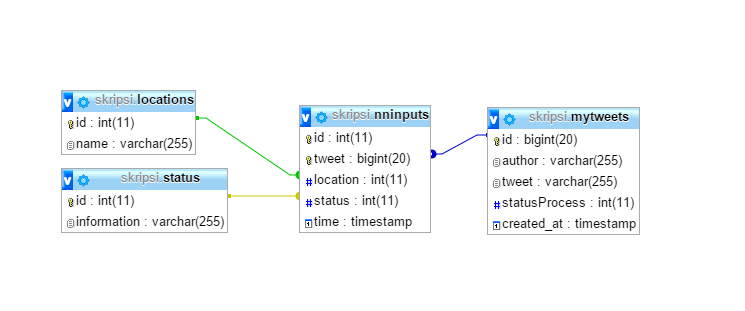
\includegraphics[width=1\linewidth]{Gambar/mine/relationalPL}
	\caption[Tabel Relational,]{Tabel Relational} 
	\label{fig:r_table}
\end{figure}}{}
\ifdefstring{\vbabd}{1}{\include{Bab/bab4}}{}
\ifdefstring{\vbabe}{1}{\include{Bab/bab5}}{}
\ifdefstring{\vbabf}{1}{\include{Bab/bab6}}{}
\ifdefstring{\vbabg}{1}{\include{Bab/bab7}}{}
\ifdefstring{\vbabh}{1}{\include{Bab/bab8}}{}
\ifdefstring{\vbabi}{1}{\include{Bab/bab9}}{}

\bibliographystyle{ieeetr}
\bibliography{pustaka}

\appendix
\apptoc

\tampillmp{\vlmp}
\ifdefstring{\vlmpa}{1}{\include{Lampiran/lampA}}{}
\ifdefstring{\vlmpb}{1}{\include{Lampiran/lampB}}{}
\ifdefstring{\vlmpc}{1}{\include{Lampiran/lampC}}{}
\ifdefstring{\vlmpd}{1}{\include{Lampiran/lampD}}{}
\ifdefstring{\vlmpe}{1}{\include{Lampiran/lampE}}{}
\ifdefstring{\vlmpf}{1}{\include{Lampiran/lampF}}{}
\ifdefstring{\vlmpg}{1}{\include{Lampiran/lampG}}{}
\ifdefstring{\vlmph}{1}{\include{Lampiran/lampH}}{}
\ifdefstring{\vlmpi}{1}{\include{Lampiran/lampI}}{}

\end{document}
